\documentclass[chaptersright]{informeutn}

\addbibresource{fuentes.bib}

\providecommand{\kHz}{\,\unit{\kilo\hertz}}
\providecommand{\MHz}{\,\unit{\mega\hertz}}

\lstdefinestyle{python}{
    backgroundcolor=\color{gray!10},
    basicstyle=\ttfamily\footnotesize,
    keywordstyle=\color{blue}\bfseries,
    stringstyle=\color{teal},
    commentstyle=\color{gray}\itshape,
    numbers=left,
    numberstyle=\tiny\color{gray},
    stepnumber=1,
    numbersep=8pt,
    frame=single,
    breaklines=true,
    breakatwhitespace=true,
    showstringspaces=false,
    captionpos=b,
    tabsize=4
}

% --- Configuración de la Carátula ---
\titulo{Trabajo Práctico de Laboratorio N° 8}
\subtitulo{Sistemas para Automatización de Mediciones. Caracterización de Circuito Resonante RLC mediante Control SCPI}
\materia{Medidas Electrónicas I}
\comision{4R2}
\autores{
    Grasso, Gaston - 401892\\
    Palombo, Franco - 401910\\
    Prieto, Angelo - 401012
}
\fecha{\today}

\begin{document}
  \maketitle
  
  \tableofcontents
  \setcounter{page}{1}
  \thispagestyle{plain}

  \chapter{Integrantes y Asignación de Roles}
De acuerdo a las normativas de la cátedra de Medidas Electrónicas I, los roles del grupo rotan en forma consecutiva
en los sucesivos trabajos prácticos. Para el presente trabajo práctico de laboratorio, la asignación formal de roles
queda establecida según se detalla en la Tabla~\ref{tab.roles:tp8}.

\begin{table}[!ht]
    \centering
    \begin{tabular}{|l|c|c|c|}
        \hline
        \textbf{Apellido y Nombres} & \textbf{Coordinador} & \textbf{Operador 1} & \textbf{Documentación} \\
                                    & \textbf{(ECG)}       & \textbf{(EO)}       & \textbf{(ED)} \\ \hline
        Prieto, Angelo & & X & \\ \hline
        Palombo, Franco & & & X \\ \hline
        Grasso, Gaston  & X & & \\ \hline
    \end{tabular}
    \caption{Tabla de asignación de roles del grupo para el Trabajo Práctico N° 8.}
    \label{tab.roles:tp8}
\end{table}

\begin{description}
    \item[Fecha de presentación estipulada:] 24 / 09 / 2026
    \item[Fecha de coloquio grupal:] 01 / 10 / 2026
\end{description}

  \chapter{Introducción}

En ensayos repetitivos o de alta densidad de datos, la operación manual del instrumental introduce
fatiga en los operadores, tiempos muertos prolongados y una dispersión estadística apreciable atribuible a demoras de
lectura y transcripción. Frente a estas limitaciones, los sistemas de medición automatizados permiten gobernar los
parámetros operativos de generadores de señal y sistemas de adquisición mediante software, garantizando secuencias de
prueba reproducibles, sincronización determinística y captura masiva de datos en tiempo real.

En este trabajo práctico se aborda el diseño e implementación de un sistema automatizado de control instrumental basado
en una computadora, interfaz RS-232 y el protocolo estandarizado SCPI (\emph{Standard Commands for Programmable
Instruments}), orientado a la caracterización experimental de la respuesta en frecuencia y el factor de calidad ($Q$) de
un circuito resonante serie RLC.

\section{Objetivos del Trabajo Práctico}
\begin{itemize}
    \item Diseñar e implementar una aplicación para el control remoto de un generador de funciones
    comercial a través de su interfaz serie RS-232 mediante comandos SCPI.
    \item Desarrollar algoritmos de barrido en frecuencia discretos, contemplando modalidades de avance automático
    con temporización configurable y avance manual con validación por teclado.
    \item Caracterizar experimentalmente la respuesta en frecuencia de un circuito resonante RLC serie provisto por la
    cátedra, identificando la frecuencia de resonancia ($f_0$) y las frecuencias de corte a $\qty{-3}{\decibel}$.
    \item Cuantificar el factor de calidad o sobretensión ($Q$) del sistema.
    \item Validar la curva de respuesta en frecuencia en el dominio de frecuencia, evaluando el impacto del ventaneo y
    el modo de persistencia infinita en pantalla.
\end{itemize}

\section{Fundamentación Teórica}

\subsection{Arquitectura de Instrumentación Programable y Protocolo SCPI}
Históricamente, la interconexión de instrumentos de prueba surgió con el bus HPIB (\emph{Hewlett-Packard Interface
Bus}), estandarizado posteriormente como IEEE-488.1 (GPIB). Dicha norma definió las especificaciones mecánicas,
eléctricas y de protocolo básico de enlace paralelo. A fin de unificar la sintaxis y los códigos de operación entre
diferentes fabricantes, se promulgaron el estándar IEEE-488.2 y la especificación SCPI (\emph{Standard Commands for
Programmable Instruments}).

La norma SCPI define una estructura de comandos basada en cadenas ASCII organizadas de forma jerárquica como un árbol.
El árbol posee un nodo raíz, del cual se desprenden trayectorias hacia nodos secundarios y nodos
hoja. La separación entre niveles jerárquicos se efectúa mediante dos puntos (\texttt{:}), y los
parámetros asociados a cada instrucción se separan del comando por un espacio en blanco. Los comandos aceptan una
forma extendida y una forma corta abreviada (resaltada en mayúsculas en los manuales de referencia):
\begin{itemize}
    \item \emph{Comandos de configuración}: Modifican un estado interno o parámetro del instrumento, por ejemplo
    \texttt{:FREQ 10000} o \texttt{:AMPL:VOLT 2.5}.
\item \emph{Comandos de consulta}: Solicitan al equipo el estado o valor de un parámetro,
    finalizando siempre con el carácter de interrogación \texttt{?}, como \texttt{:FREQ?} o \texttt{*IDN?}.
    \item \emph{Comandos comunes IEEE-488.2}: Comienzan con un asterisco y realizan acciones globales
    predefinidas: \texttt{*RST} (reinicio a condiciones de fábrica), \texttt{*IDN?} (consulta de fabricante, modelo,
    número de serie y versión de firmware) y \texttt{*CLS} (borrado de registros de estado).
\end{itemize}

\subsection{Teoría del Circuito Resonante Serie RLC}
Un circuito resonante serie está compuesto por una resistencia total equivalente $R_{\text{tot}}$, una inductancia
concentrada $L$ y una capacitancia $C$, excitados por una fuente senoidal de tensión $v_s(t) = V_s \cos(\omega t)$.
La impedancia compleja equivalente del conjunto vista desde los bornes de la fuente se expresa como:
\begin{equation}
    Z(j\omega) = R_{\text{tot}} + j \left( \omega L - \frac{1}{\omega C} \right)
    \label{eq.ej1:impedancia}
\end{equation}
donde $R_{\text{tot}}$ engloba tanto las resistencias explícitas del circuito como la resistencia interna del
generador ($R_g$) y las pérdidas óhmicas parásitas del devanado de la bobina ($R_L$).

La condición de resonancia serie se produce en $\omega_0$ en la cual la reactancia inductiva
$X_L = \omega L$ cancela con exactitud a la reactancia capacitiva $X_C = \frac{1}{\omega C}$, anulando la parte
imaginaria de la impedancia:
\begin{equation}
    \omega_0 L - \frac{1}{\omega_0 C} = 0 \implies \omega_0 = \frac{1}{\sqrt{LC}}
    \label{eq.ej1:w0}
\end{equation}
Por consiguiente, la frecuencia de resonancia teórica en Hertz queda determinada por la relación de Thomson:
\begin{equation}
    f_0 = \frac{1}{2 \pi \sqrt{L C}}
    \label{eq.ej1:fres}
\end{equation}

A la frecuencia $f_0$, el circuito manifiesta las siguientes propiedades singulares:
\begin{enumerate}
    \item La impedancia total alcanza su valor mínimo absoluto y puramente resistivo: $Z(j\omega_0) = R_{\text{tot}}$.
    \item La corriente que circula por la malla adquiere su módulo máximo: $I_0 = \frac{V_s}{R_{\text{tot}}}$,
    encontrándose en fase con la tensión de excitación ($\Delta \varphi = 0^\circ$).
    \item Las caídas de tensión en los componentes reactivos individuales ($v_L$ y $v_C$) presentan una magnitud que
    puede superar ampliamente el valor de la tensión de entrada $V_s$. Este fenómeno se denomina sobretensión o
    resonancia de tensión.
\end{enumerate}

\subsection{Factor de Calidad y Relación con el Ancho de Banda}
El factor de calidad $Q$ (o factor de selectividad) cuantifica la relación entre la energía reactiva almacenada en el
sistema y la energía activa disipada por ciclo en los elementos resistivos. Para una malla resonante serie, se define
como:
\begin{equation}
    Q = \frac{\omega_0 L}{R_{\text{tot}}} = \frac{1}{\omega_0 C R_{\text{tot}}} = \frac{1}{R_{\text{tot}}} \sqrt{\frac{L}{C}}
    \label{eq.ej1:q_definicion}
\end{equation}

Analizando la caída de tensión en bornes del capacitor a la frecuencia de resonancia:
\begin{equation}
    V_C(\omega_0) = I_0 \cdot X_C(\omega_0) = \left( \frac{V_s}{R_{\text{tot}}} \right) \left( \frac{1}{\omega_0 C} \right) = Q \cdot V_s
    \label{eq.ej1:magnificacion}
\end{equation}
La ecuación~\eqref{eq.ej1:magnificacion} evidencia que la relación entre la tensión pico a pico en el capacitor y la
tensión total aplicada a la rama serie en resonancia proporciona una estimación directa del factor de calidad del
sistema, denominado factor de sobretensión:
\begin{equation}
    Q_v = \frac{V_C(f_0)}{V_{\text{in}}(f_0)}
    \label{eq.ej1:qv}
\end{equation}

Por otra parte, si se analiza la curva de transferencia en función de la frecuencia, se definen las frecuencias de
corte inferior ($f_1$ o $f_{\text{inf}}$) y superior ($f_2$ o $f_{\text{sup}}$) como aquellos puntos donde la potencia
entregada cae a la mitad de su valor de resonancia ($\qty{-3}{\decibel}$ respecto al máximo). En dichos puntos, la
tensión en el capacitor se reduce a un factor $1/\sqrt{2} \approx 0.7071$ del valor pico:
\begin{equation}
    V_C(f_1) = V_C(f_2) = \frac{V_C(f_0)}{\sqrt{2}}
    \label{eq.ej1:umbral_3db}
\end{equation}

El ancho de banda a $\qty{-3}{\decibel}$ se define como la diferencia entre ambas frecuencias de corte:
\begin{equation}
    \Delta f = f_{\text{sup}} - f_{\text{inf}}
    \label{eq.ej1:bw}
\end{equation}
El factor de calidad experimental derivado de la selectividad en frecuencia resulta entonces:
\begin{equation}
    Q_{\Delta f} = \frac{f_0}{\Delta f}
    \label{eq.ej1:q_bw}
\end{equation}


  \chapter{Materiales e Instrumental}

Para el desarrollo experimental de las rutinas de comunicación remota, el control automatizado del barrido en
frecuencia y la caracterización circuital del banco RLC, se dispuso del siguiente equipamiento de laboratorio,
instrumentos de medición y componentes electrónicos:

\begin{itemize}
    \item Generador de Funciones GW-Instek GFG-3015 (G-168)
    \item Osciloscopio Digital Tektronix TDS 1001 (O-162)
    \item Puntas de Prueba Pasivas Compensadas
    \item Cable de Disparo BNC-BNC
    \item Placa de Ensayos RLC
    \item Adaptador USB a Serie RS-232
    \item Computadora Portátil de Control
\end{itemize}

  \chapter{Desarrollo Experimental y Análisis de Resultados}

\section{Configuración del Banco Circuital y Asignación de Canales}
La topología circuital completa, incluyendo el generador de funciones, la resistencia
limitadora de protección, los puntos de toma de señal y las conexiones hacia el osciloscopio digital, se ilustra en el
esquemático de la Figura~\ref{crkt.ej1:rlc}. Asimismo, en la Figura~\ref{fig.ej1:crkt_board} se observa el montaje
físico de los componentes sobre la mesa de laboratorio.

\begin{figure}[!ht]
    \centering
    \begin{tikzpicture}[scale=0.92, transform shape, >=stealth]

    % ========================================================
    % 1. GENERADOR DE FUNCIONES (GW-Instek GFG-3015)
    % ========================================================
    \draw[thick, fill=gray!8] (-0.6, 0.2) rectangle (3.2, 5.0);
    \node[font=\bfseries\small, align=center] at (1.2, 2.7) {Generador de\\Funciones\\[5pt]\footnotesize GW-Instek\\GFG-3015};
    
    % Conectores BNC panel frontal (x = 3.2)
    \coordinate (gen_out)  at (3.2, 4.2);
    \coordinate (gen_sync) at (3.2, 1.2);
    \coordinate (gen_gnd)  at (3.2, 0.2);
    
    \draw[fill=white, thick] (gen_out) circle (3.5pt);
    \node[left=4pt, font=\scriptsize\bfseries] at (gen_out) {MAIN OUT};
    
    \draw[fill=white, thick] (gen_sync) circle (3.5pt);
    \node[left=4pt, font=\scriptsize\bfseries] at (gen_sync) {SYNC OUT};

    \draw (1.3, 0.2) node[ground]{};

    % ========================================================
    % 2. OSCILOSCOPIO DIGITAL (Tektronix TDS 1001)
    % ========================================================
    \draw[thick, fill=gray!8] (11.0, 0.2) rectangle (14.8, 5.0);
    \node[font=\bfseries\small, align=center] at (13.0, 2.7) {Osciloscopio\\Digital\\[5pt]\footnotesize Tektronix\\TDS 1001};

    % Conectores BNC panel frontal (x = 11.0)
    \coordinate (osc_ch1)  at (11.0, 4.2);
    \coordinate (osc_ch2)  at (11.0, 2.1);
    \coordinate (osc_trig) at (11.0, 1.2);
    \coordinate (osc_gnd)  at (11.0, 0.2);
    
    \draw[fill=white, thick] (osc_ch1) circle (3.5pt);
    \node[right=4pt, font=\scriptsize\bfseries, color=blue!80!black] at (osc_ch1) {CH1};
    
    \draw[fill=white, thick] (osc_ch2) circle (3.5pt);
    \node[right=4pt, font=\scriptsize\bfseries, color=red!80!black] at (osc_ch2) {CH2};
    
    \draw[fill=white, thick] (osc_trig) circle (3.5pt);
    \node[right=4pt, font=\scriptsize\bfseries] at (osc_trig) {EXT TRIG};

    \draw (12.9, 0.2) node[ground]{};

    % ========================================================
    % 3. BANCO DE PRUEBA RLC (Placa MEI)
    % ========================================================
    \def\xBranch{6.8}
    
    % Resistor serie de protección r = 47 ohm (con separación holgada hacia Nodo A)
    \draw (gen_out) to[short] (4.0, 4.2)
          to[R, l={$r = \qty{47}{\ohm}$}, *-*] (5.8, 4.2)
          -- (\xBranch, 4.2) coordinate (nodeA);
    \node[above=4pt, font=\scriptsize\bfseries, color=blue!85!black] at (nodeA) {Nodo A};

    % Rama resonante vertical: Inductor L + Resistencia interna RL
    \draw (nodeA) to[L, l_={$L = \qty{30}{\milli\henry}$}] (\xBranch, 3.2)
          to[R, l_={$R_L$}] (\xBranch, 2.3)
          -- (\xBranch, 2.1) coordinate (nodeB);
    \node[left=5pt, font=\scriptsize\bfseries, color=red!85!black] at (nodeB) {Nodo B};

    % Capacitor C a masa
    \draw (nodeB) to[C, l_={$C = \qty{7}{\nano\farad}$}, *-*] (\xBranch, 0.9) coordinate (nodeGndRLC);
    
    % Conexión a la línea de masa común
    \draw (nodeGndRLC) -- (\xBranch, 0.2);
    \draw (\xBranch, 0.2) node[ground]{};

    % ========================================================
    % 4. CONEXIÓN DE PUNTAS Y REFERENCIAS (CH1, CH2, DISPARO)
    % ========================================================
    
    % CANAL 1 (CH1): Mide e_tot en Nodo A
    \draw[blue!85!black, very thick] (nodeA) -- (osc_ch1);
    \node[above=3pt, font=\footnotesize\bfseries, color=blue!85!black] 
        at ($(\xBranch, 4.2)!0.55!(osc_ch1)$) {$e_{\text{tot}}$ (Canal 1)};
    \draw[blue!85!black, fill=blue!85!black] (nodeA) circle (2.5pt);

    % CANAL 2 (CH2): Mide e_c en Nodo B
    \draw[red!85!black, very thick] (nodeB) -- (osc_ch2);
    \node[above=3pt, font=\footnotesize\bfseries, color=red!85!black] 
        at ($(\xBranch, 2.1)!0.55!(osc_ch2)$) {$e_c$ (Canal 2)};
    \draw[red!85!black, fill=red!85!black] (nodeB) circle (2.5pt);

    % LÍNEA DE MASA COMÚN
    \draw[black, thick] (gen_gnd) -- (osc_gnd);

    % DISPARO EXTERNO (SYNC -> EXT TRIG): Por debajo de la masa
    \draw[gray!50!black, thick, dashed] (gen_sync) -- ++(0.4, 0) -- ++(0, -1.8)
          -- ($(osc_trig) + (-0.4, -1.8)$)
          node[midway, below=2pt, font=\scriptsize\bfseries] {Sincronismo TTL (\emph{Sync Out} $\to$ \emph{Ext Trig})}
          -- ++(0, 1.8) -- (osc_trig);

\end{tikzpicture}

    \caption{Esquema eléctrico del circuito de ensayo y conexionado de instrumentos.}
    \label{crkt.ej1:rlc}
\end{figure}

\begin{figure}[!ht]
    \centering
    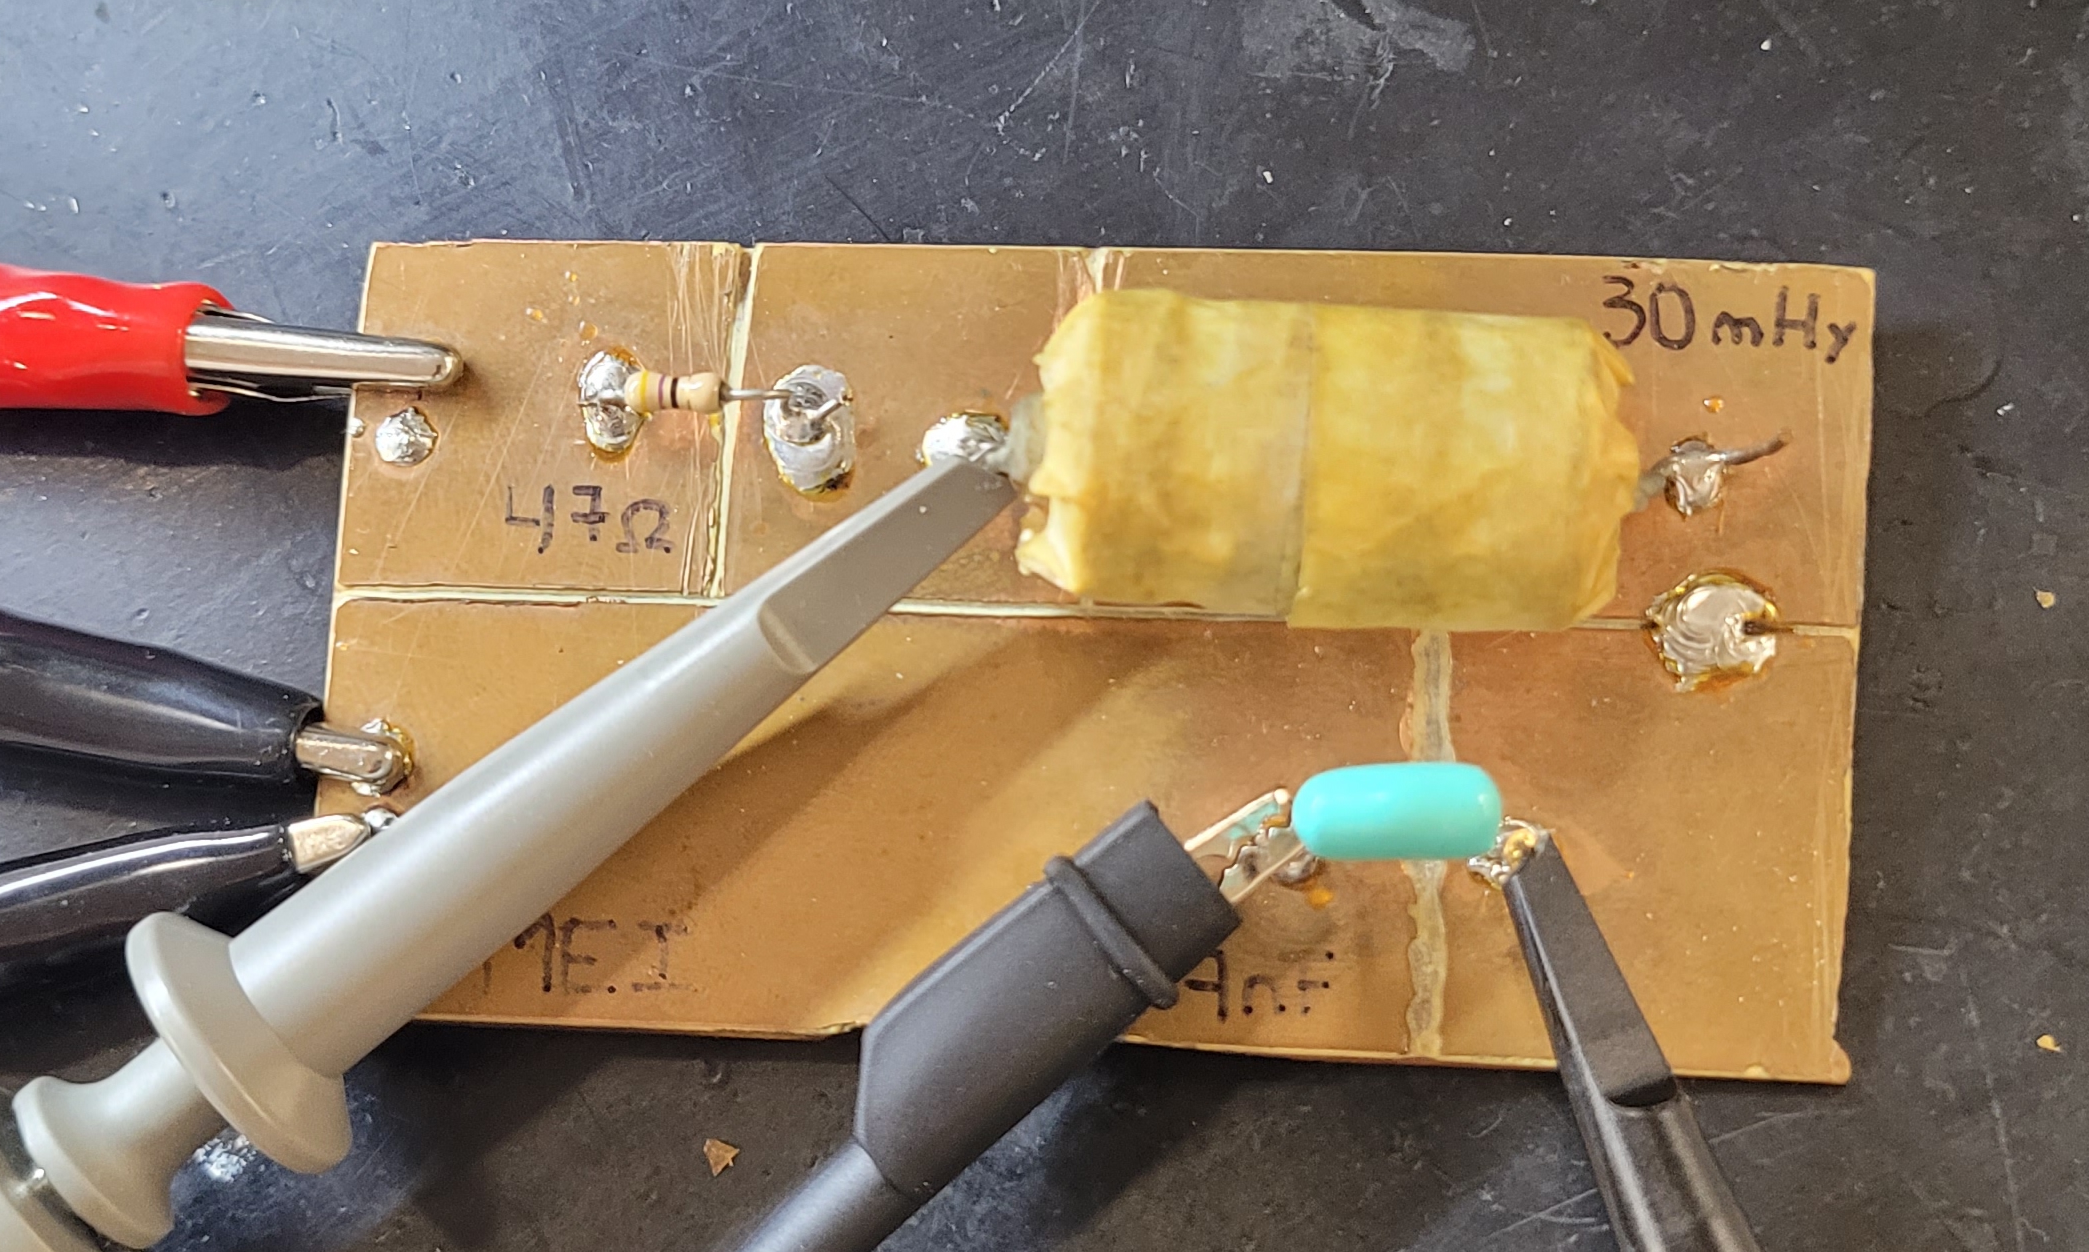
\includegraphics[width=0.65\textwidth]{pictures/crkt_rlc.jpeg}
    \caption{Placa de circuito impreso del banco RLC bajo ensayo en laboratorio.}
    \label{fig.ej1:crkt_board}
\end{figure}

El circuito cuenta con una resistencia serie de valor nominal $r = \qty{47}{\ohm}$, cuya función primordial consiste
en preservar la integridad del amplificador de salida del generador de funciones. Dado que en la condición de resonancia
la impedancia reactiva equivalente del par LC se anula teóricamente ($X_L - X_C = 0$), sin la presencia de este
resistor la impedancia de carga vista por la fuente caería exclusivamente a las pérdidas parásitas del inductor,
provocando una corriente excesiva y distorsión por sobrecarga.

\section{Implementación del Software de Control SCPI en Python}
A fin de comandar el generador de funciones de forma automatizada, se desarrolló un script en Python
(\texttt{controlador\_generador\_funciones.py}) utilizando la biblioteca \texttt{pySerial}.

\begin{figure}[!ht]
    \centering
    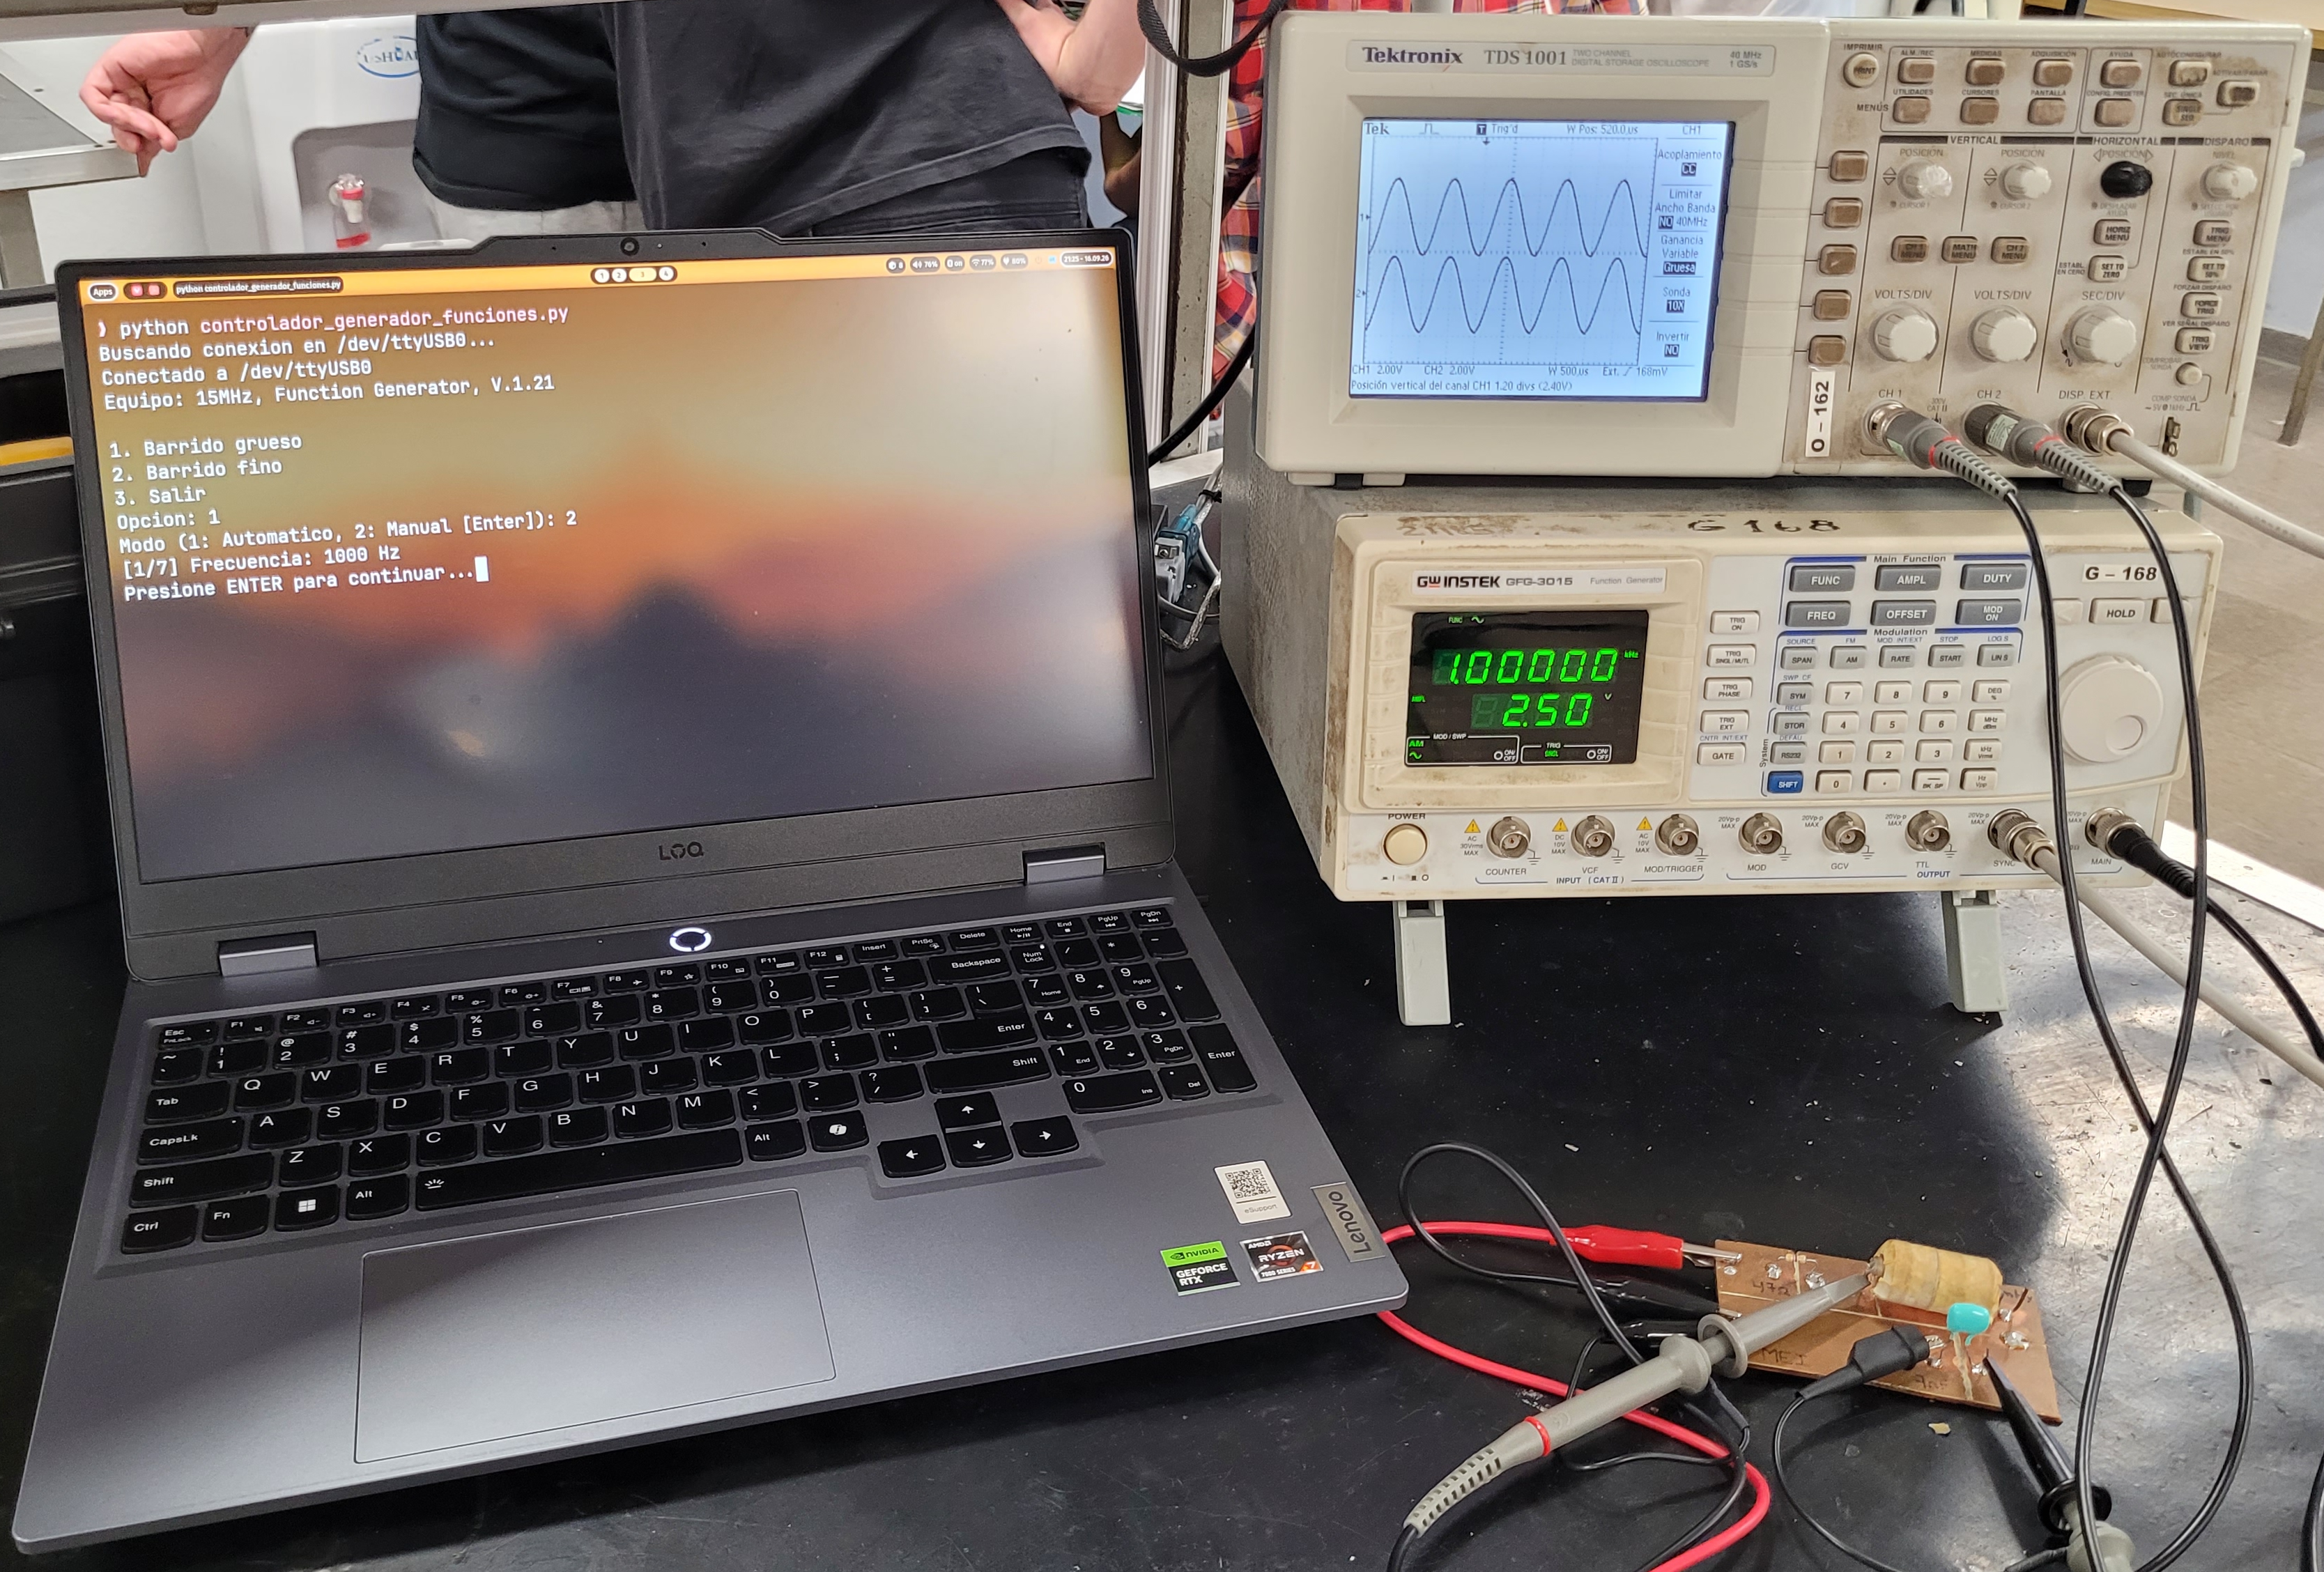
\includegraphics[width=0.75\textwidth]{pictures/setup_apk.jpeg}
    \caption{Computadora ejecutando el programa de control.}
    \label{fig.ej1:setup_apk}
\end{figure}

El flujo del software se estructura en tres etapas funcionales:
\begin{enumerate}
    \item \emph{Apertura de puerto y verificación de enlace:} El programa abre el puerto serie virtual asignado a
    \texttt{/dev/ttyUSB0} con una tasa de transferencia de $\qty{9600}{\text{baud}}$, 8 bits de datos, sin paridad y
    1 bit de parada. A continuación, envía la instrucción de identificación IEEE-488.2:
    \[
        \texttt{*IDN?\textbackslash n}
    \]
    El generador respondió satisfactoriamente devolviendo la trama ASCII:
    \[
        \texttt{"15MHz, Function Generator, V.1.21"}
    \]
    lo cual validó el correcto funcionamiento del enlace físico RS-232 y el intérprete de comandos.
    \item \emph{Inicialización y configuración de parámetros de señal:} Antes de iniciar cualquier barrido, la rutina
    \texttt{gen\_setup()} transmite la secuencia de comandos SCPI requerida:
    \begin{itemize}
        \item \texttt{:FUNC:WAV 1}: Selecciona forma de onda senoidal pura.
        \item \texttt{:AMPL:UNIT 1}: Fija la unidad de amplitud en voltios pico a pico ($\mathrm{V_{pp}}$).
        \item \texttt{:AMPL:VOLT 2.5}: Configura la amplitud de salida en $\qty{2.5}{\volt}$. Debido a que el
        generador calibra internamente su escala considerando una carga terminada en $\qty{50}{\ohm}$, al trabajar
        sobre la impedancia significativamente más elevada del circuito RLC, la fuerza electromotriz entregada a circuito
        abierto resulta de $\qty{5.0}{\volt_{\text{pp}}}$.
        \item \texttt{:OFFSet 0}: Anula cualquier componente de continua (\emph{offset} nulo).
    \end{itemize}
    \item \emph{Ejecución de barridos de frecuencia:} El operador puede seleccionar entre una modalidad de barrido
    grueso (con puntos normalizados prefijados) o barrido fino (definiendo frecuencia inicial, final y paso de avance).
    Asimismo, el script permite optar por avance automático (con un retardo en segundos por escalón) o manual mediante
    la tecla \texttt{ENTER}, permitiendo estabilizar las lecturas y capturar registros fotográficos.
\end{enumerate}

\section{Barrido Grueso en Frecuencia (1 kHz a 100 kHz)}
La primera actividad experimental consistió en ejecutar un barrido grueso en frecuencia con saltos amplios, con el
propósito de relevar cualitativamente la curva de respuesta y acotar el entorno donde se ubica la resonancia del sistema.
Las frecuencias especificadas por la consigna fueron: $\qty{1}{\kilo\hertz}$, $\qty{2}{\kilo\hertz}$, $\qty{5}{\kilo\hertz}$,
$\qty{10}{\kilo\hertz}$, $\qty{20}{\kilo\hertz}$, $\qty{50}{\kilo\hertz}$ y $\qty{100}{\kilo\hertz}$.

\begin{figure}[!ht]
    \centering
    \begin{subfigure}[t]{0.48\textwidth}
        \centering
        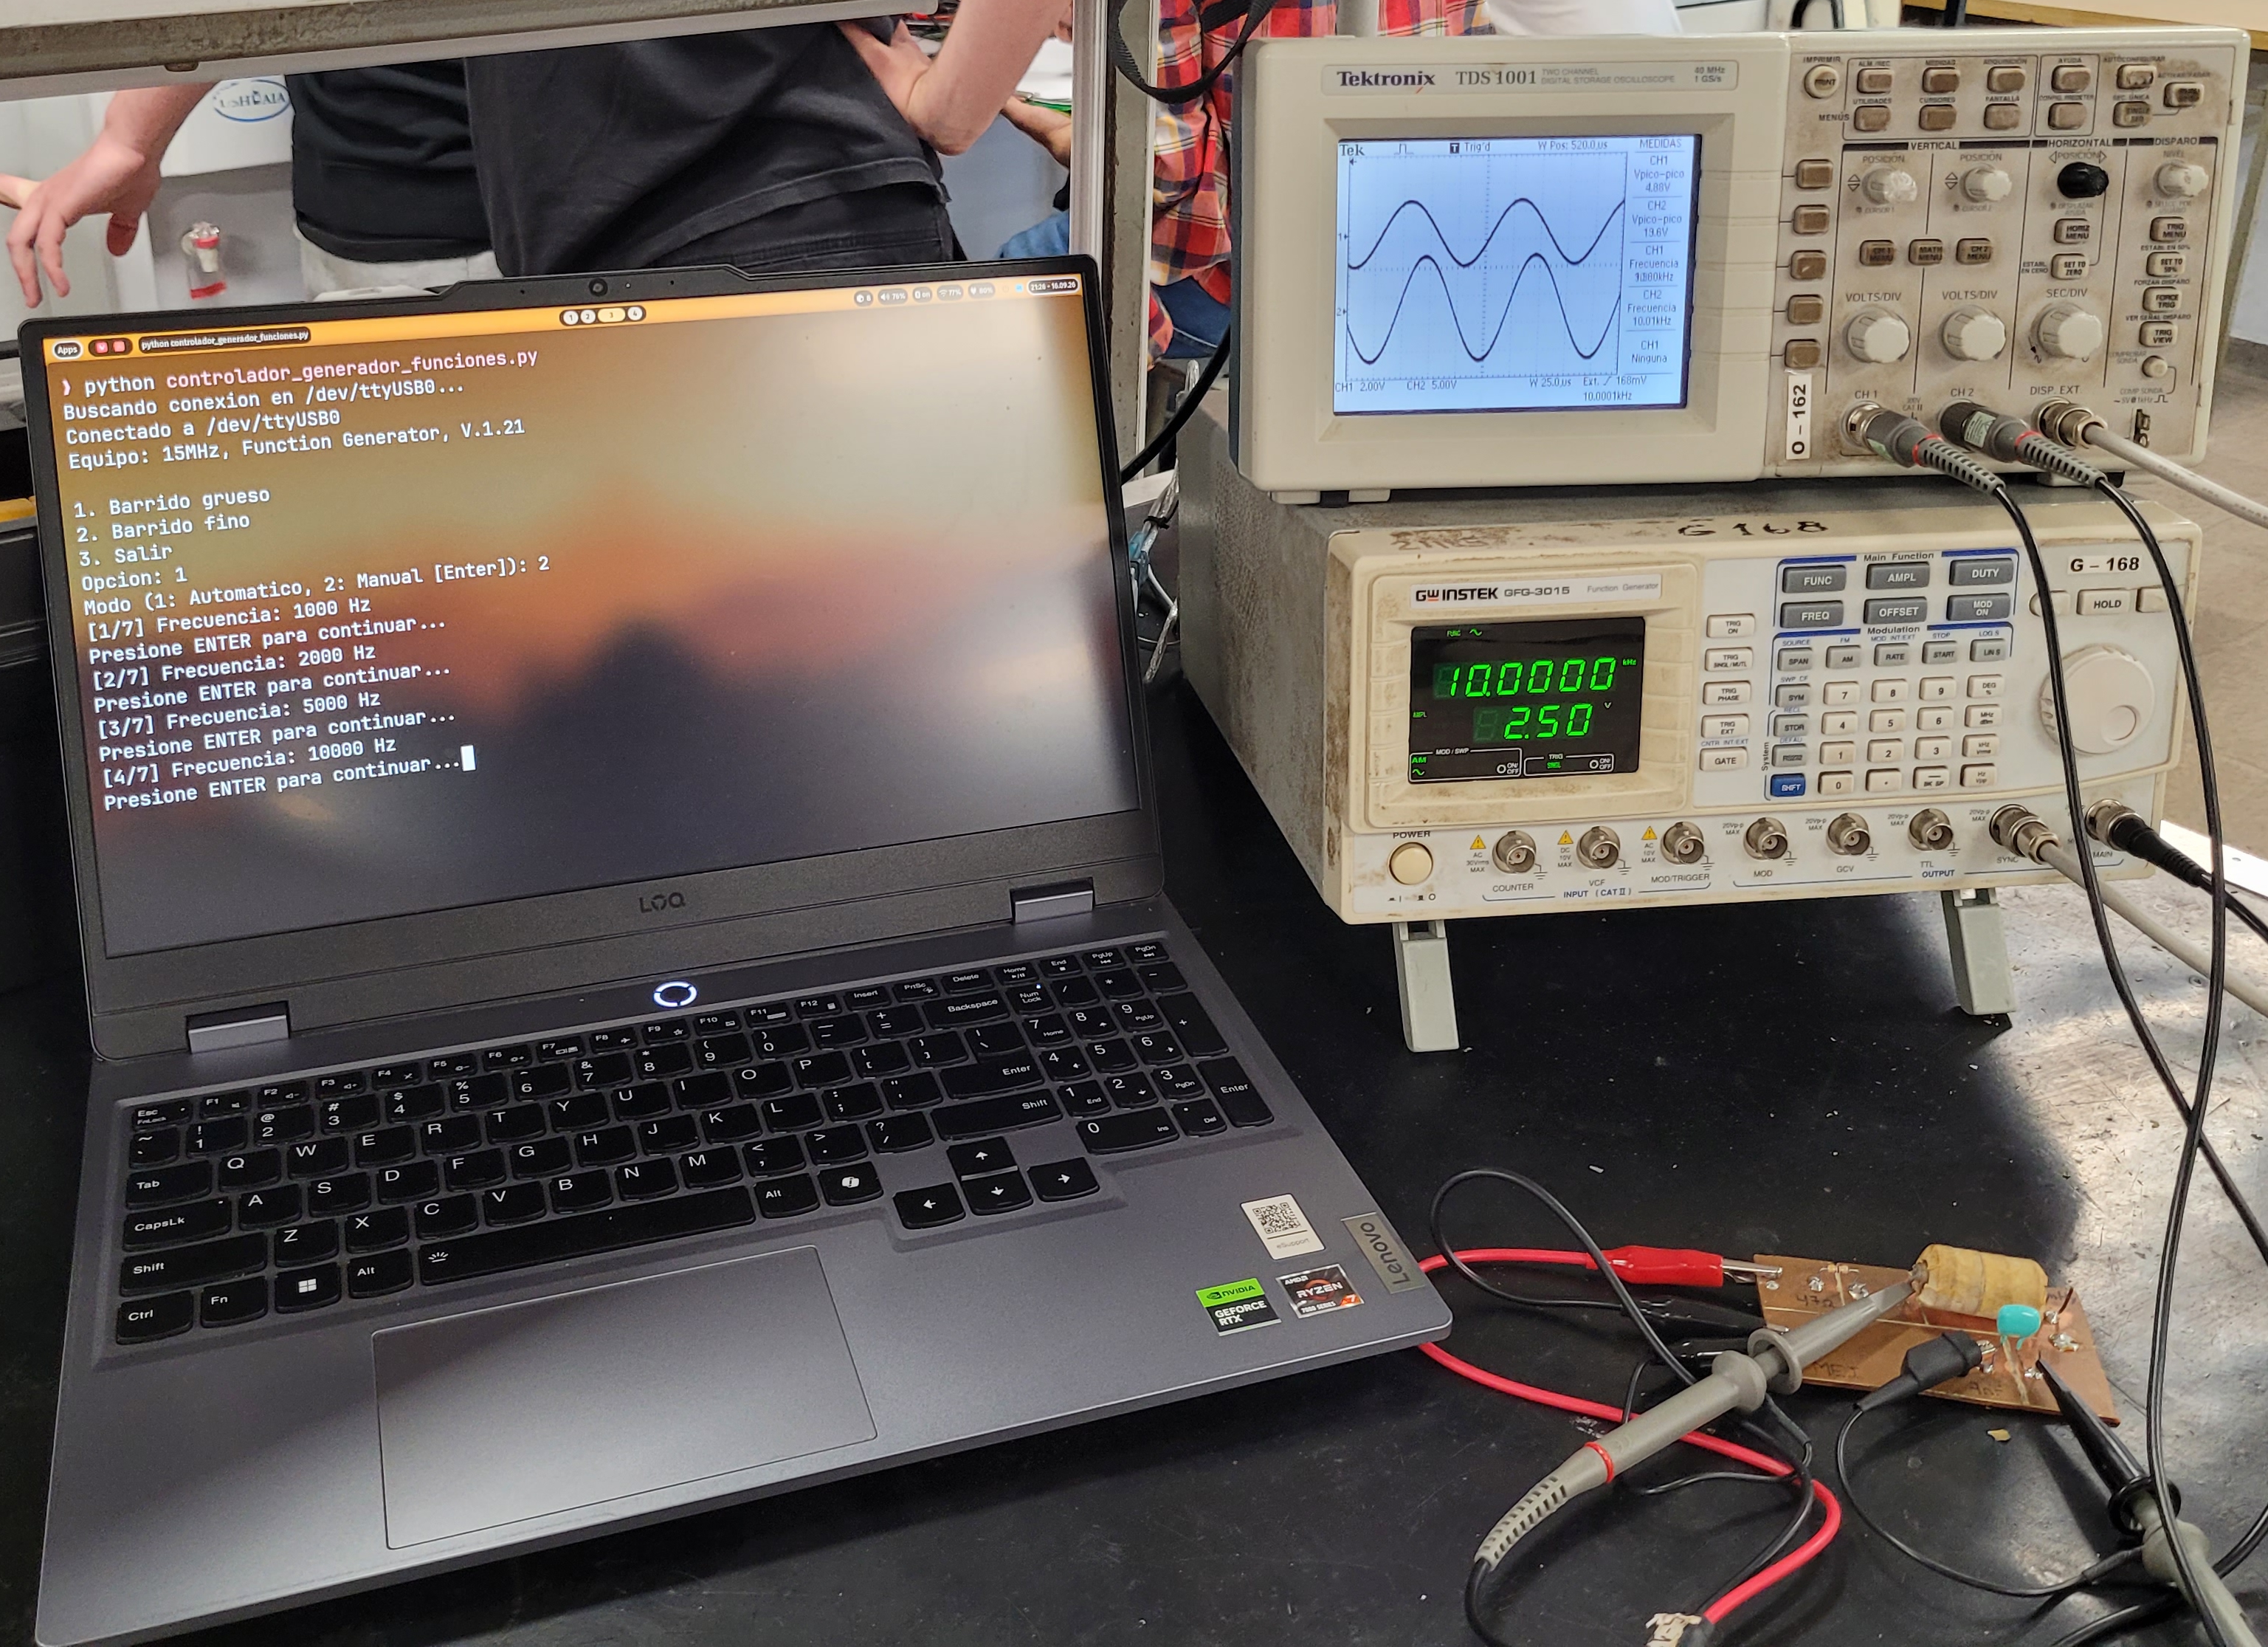
\includegraphics[width=\textwidth]{pictures/setup_grueso_f0.jpeg}
        \caption{Consola de control en paso $\qty{10}{\kilo\hertz}$.}
        \label{fig.ej1:setup_grueso}
    \end{subfigure}
    \hfill
    \begin{subfigure}[t]{0.48\textwidth}
        \centering
        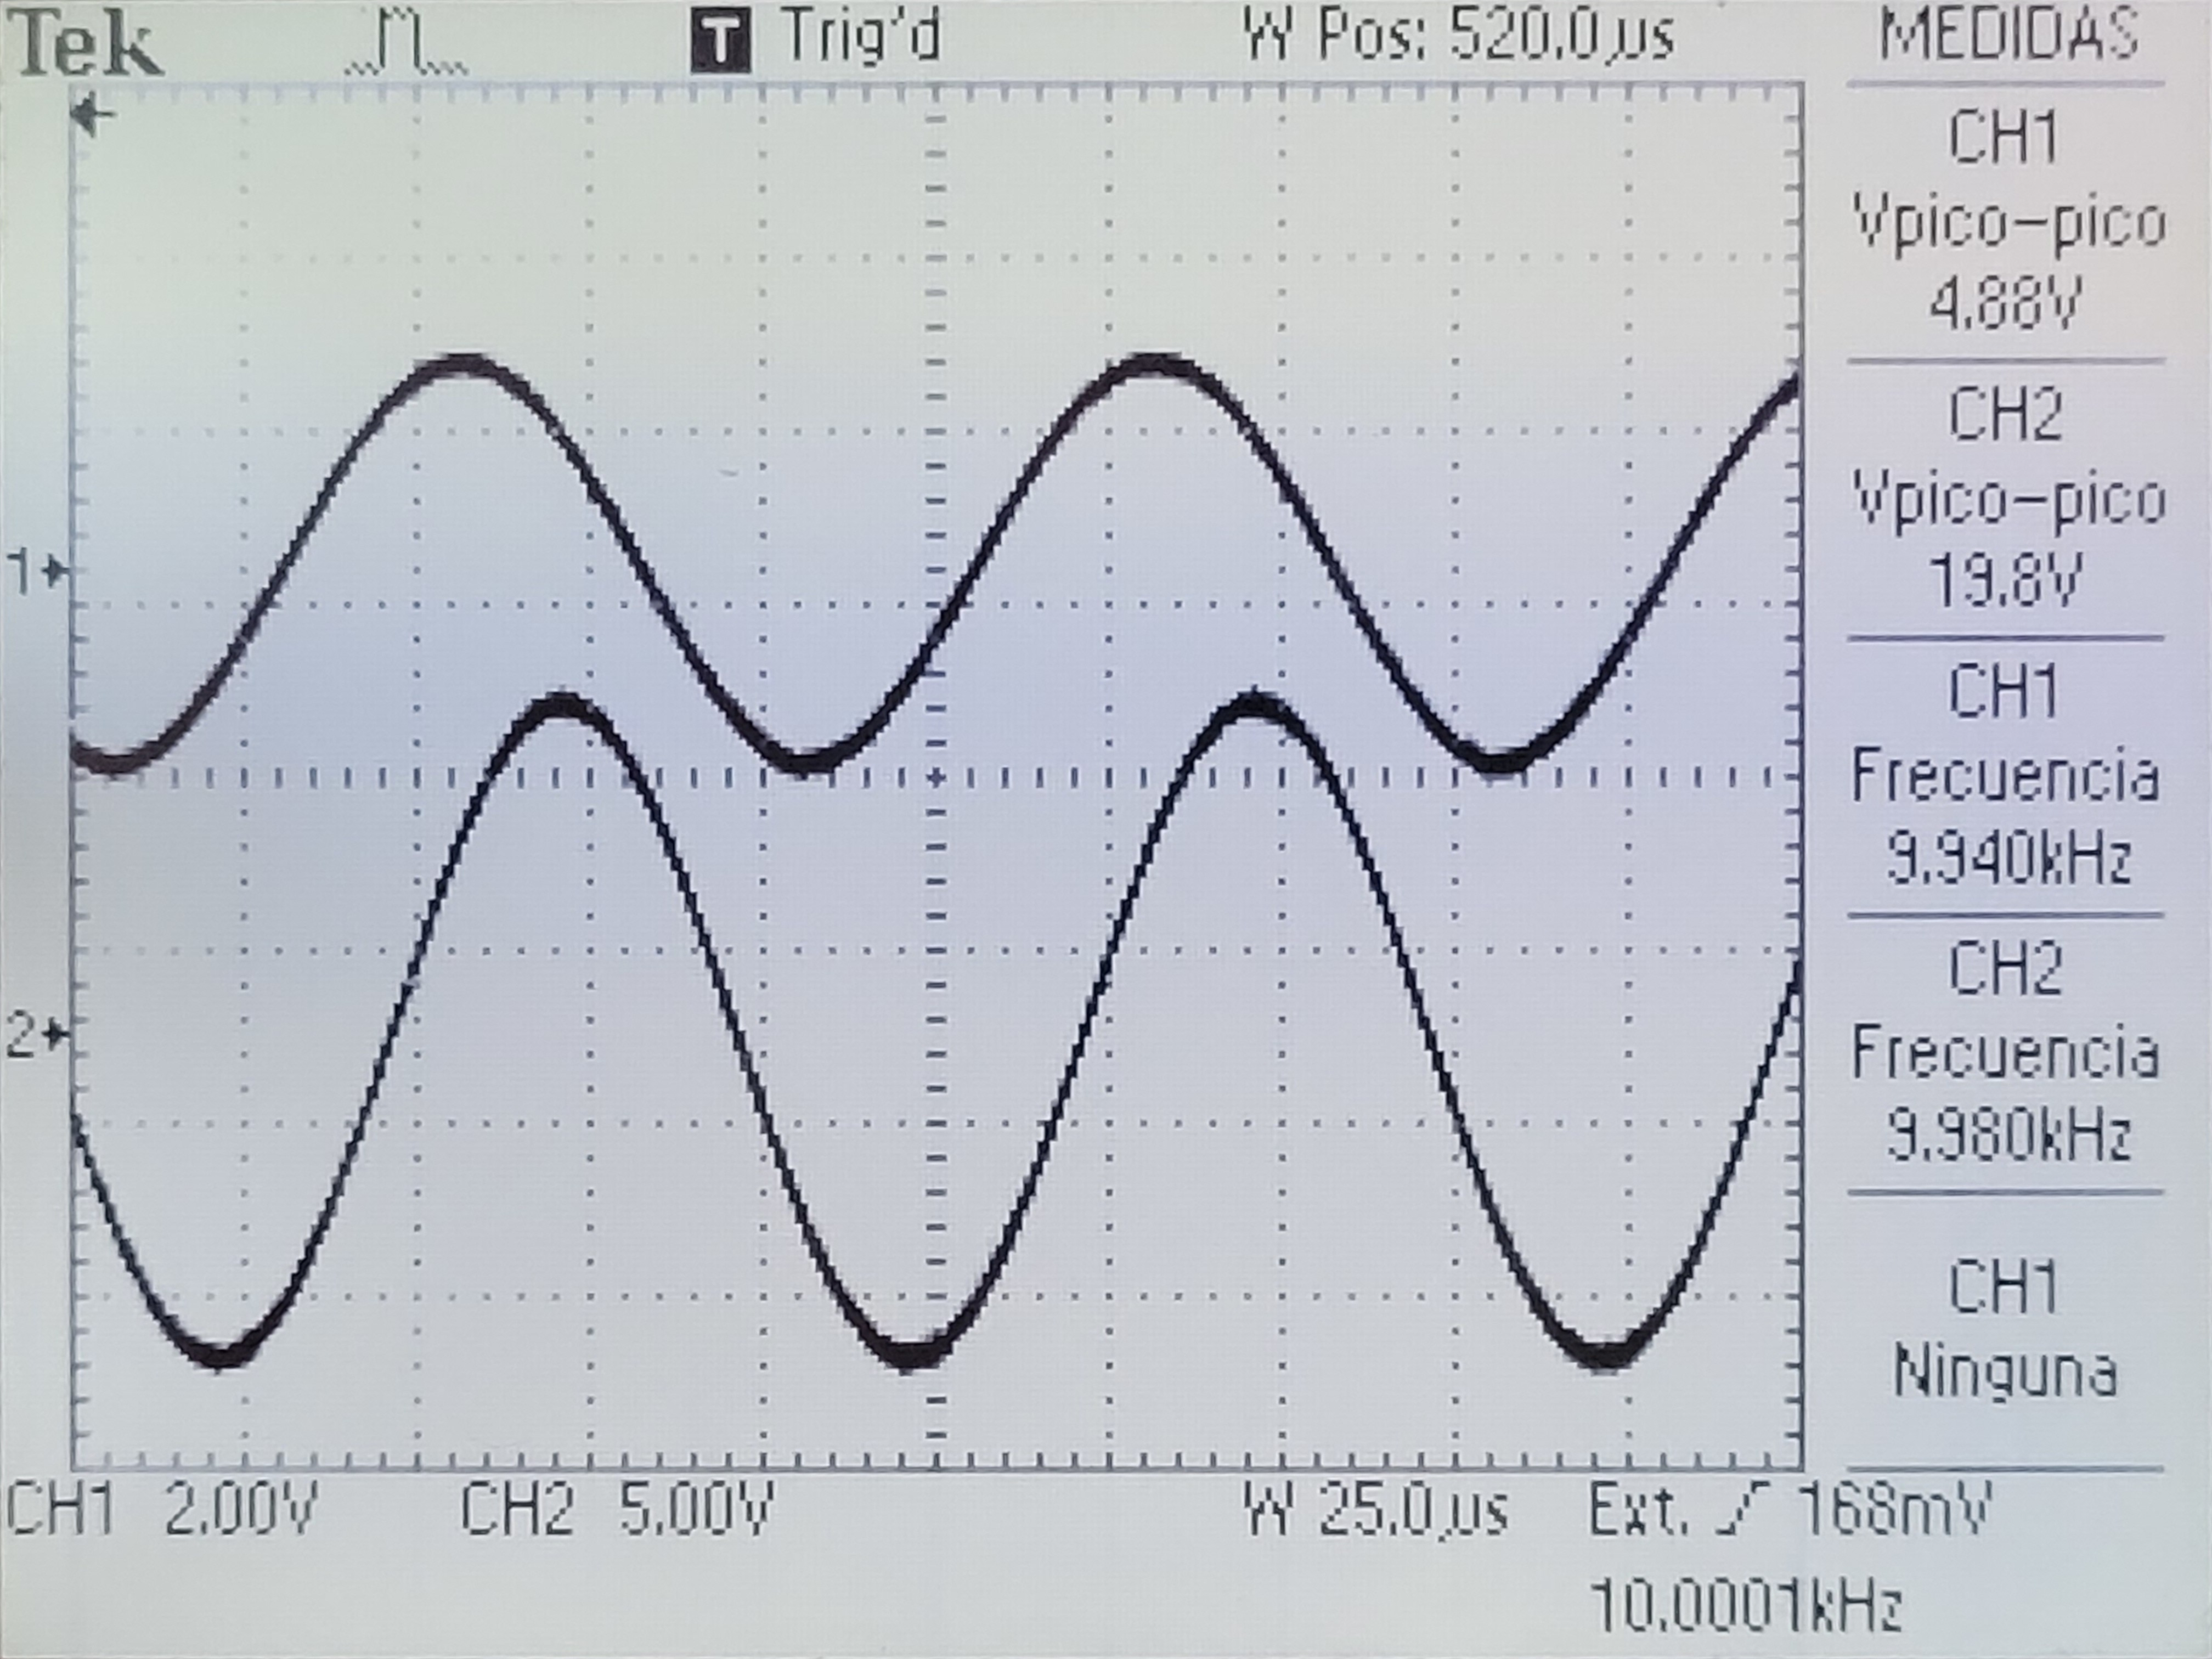
\includegraphics[width=\textwidth]{pictures/osc_grueso_f0.jpeg}
        \caption{Captura del osciloscopio en $\qty{10}{\kilo\hertz}$.}
        \label{fig.ej1:osc_grueso}
    \end{subfigure}
    \caption{Ensayo de barrido grueso en el punto de resonancia aproximada ($\qty{10}{\kilo\hertz}$).}
    \label{fig.ej1:barrido_grueso}
\end{figure}

Durante la progresión del barrido, se observó que a frecuencias bajas ($\qtyrange{1}{5}{\kilo\hertz}$), la reactancia
capacitiva predomina holgadamente sobre la inductiva ($X_C \gg X_L$), por lo que la corriente en la malla es reducida y
la tensión en el capacitor reproduce aproximadamente la tensión de entrada. Al aproximarse a $\qty{10}{\kilo\hertz}$,
se manifestó un incremento abrupto de la amplitud debido a la proximidad del polo de resonancia:
\begin{itemize}
    \item Tensión total aplicada: $V_{\text{pp}} = \qty{4.88}{\volt}$.
    \item Tensión en el capacitor: $V_{\text{pp}} = \qty{19.8}{\volt}$.
\end{itemize}
A frecuencias superiores ($\qtyrange{20}{100}{\kilo\hertz}$), la reactancia inductiva se torna dominante ($X_L \gg X_C$),
elevando la impedancia total y atenuando progresivamente la tensión transferida al capacitor hasta valores despreciables.
Este ensayo confirmó de manera concluyente que la frecuencia de resonancia se ubica en las inmediaciones de los
$\qty{10}{\kilo\hertz}$.

\section{Barrido Fino y Localización de Frecuencias Singulares}
Con la zona de interés delimitada, se procedió a configurar barridos finos con incrementos menores a fin de identificar
con precisión:
\begin{enumerate}
    \item La frecuencia de resonancia exacta ($f_0$) y la tensión máxima sobre el capacitor ($V_{C,\text{max}}$).
    \item La frecuencia de corte inferior ($f_{\text{inf}}$) y superior ($f_{\text{sup}}$) correspondientes al nivel
    de $\qty{-3}{\decibel}$ respecto al pico de resonancia.
\end{enumerate}

\subsection{Identificación del Pico de Resonancia (\texorpdfstring{$f_0$}{f0})}
Efectuando un barrido fino en torno a $\qty{10}{\kilo\hertz}$, ajustamos la frecuencia del generador hasta maximizar la
amplitud pico a pico.

\begin{figure}[!ht]
    \centering
    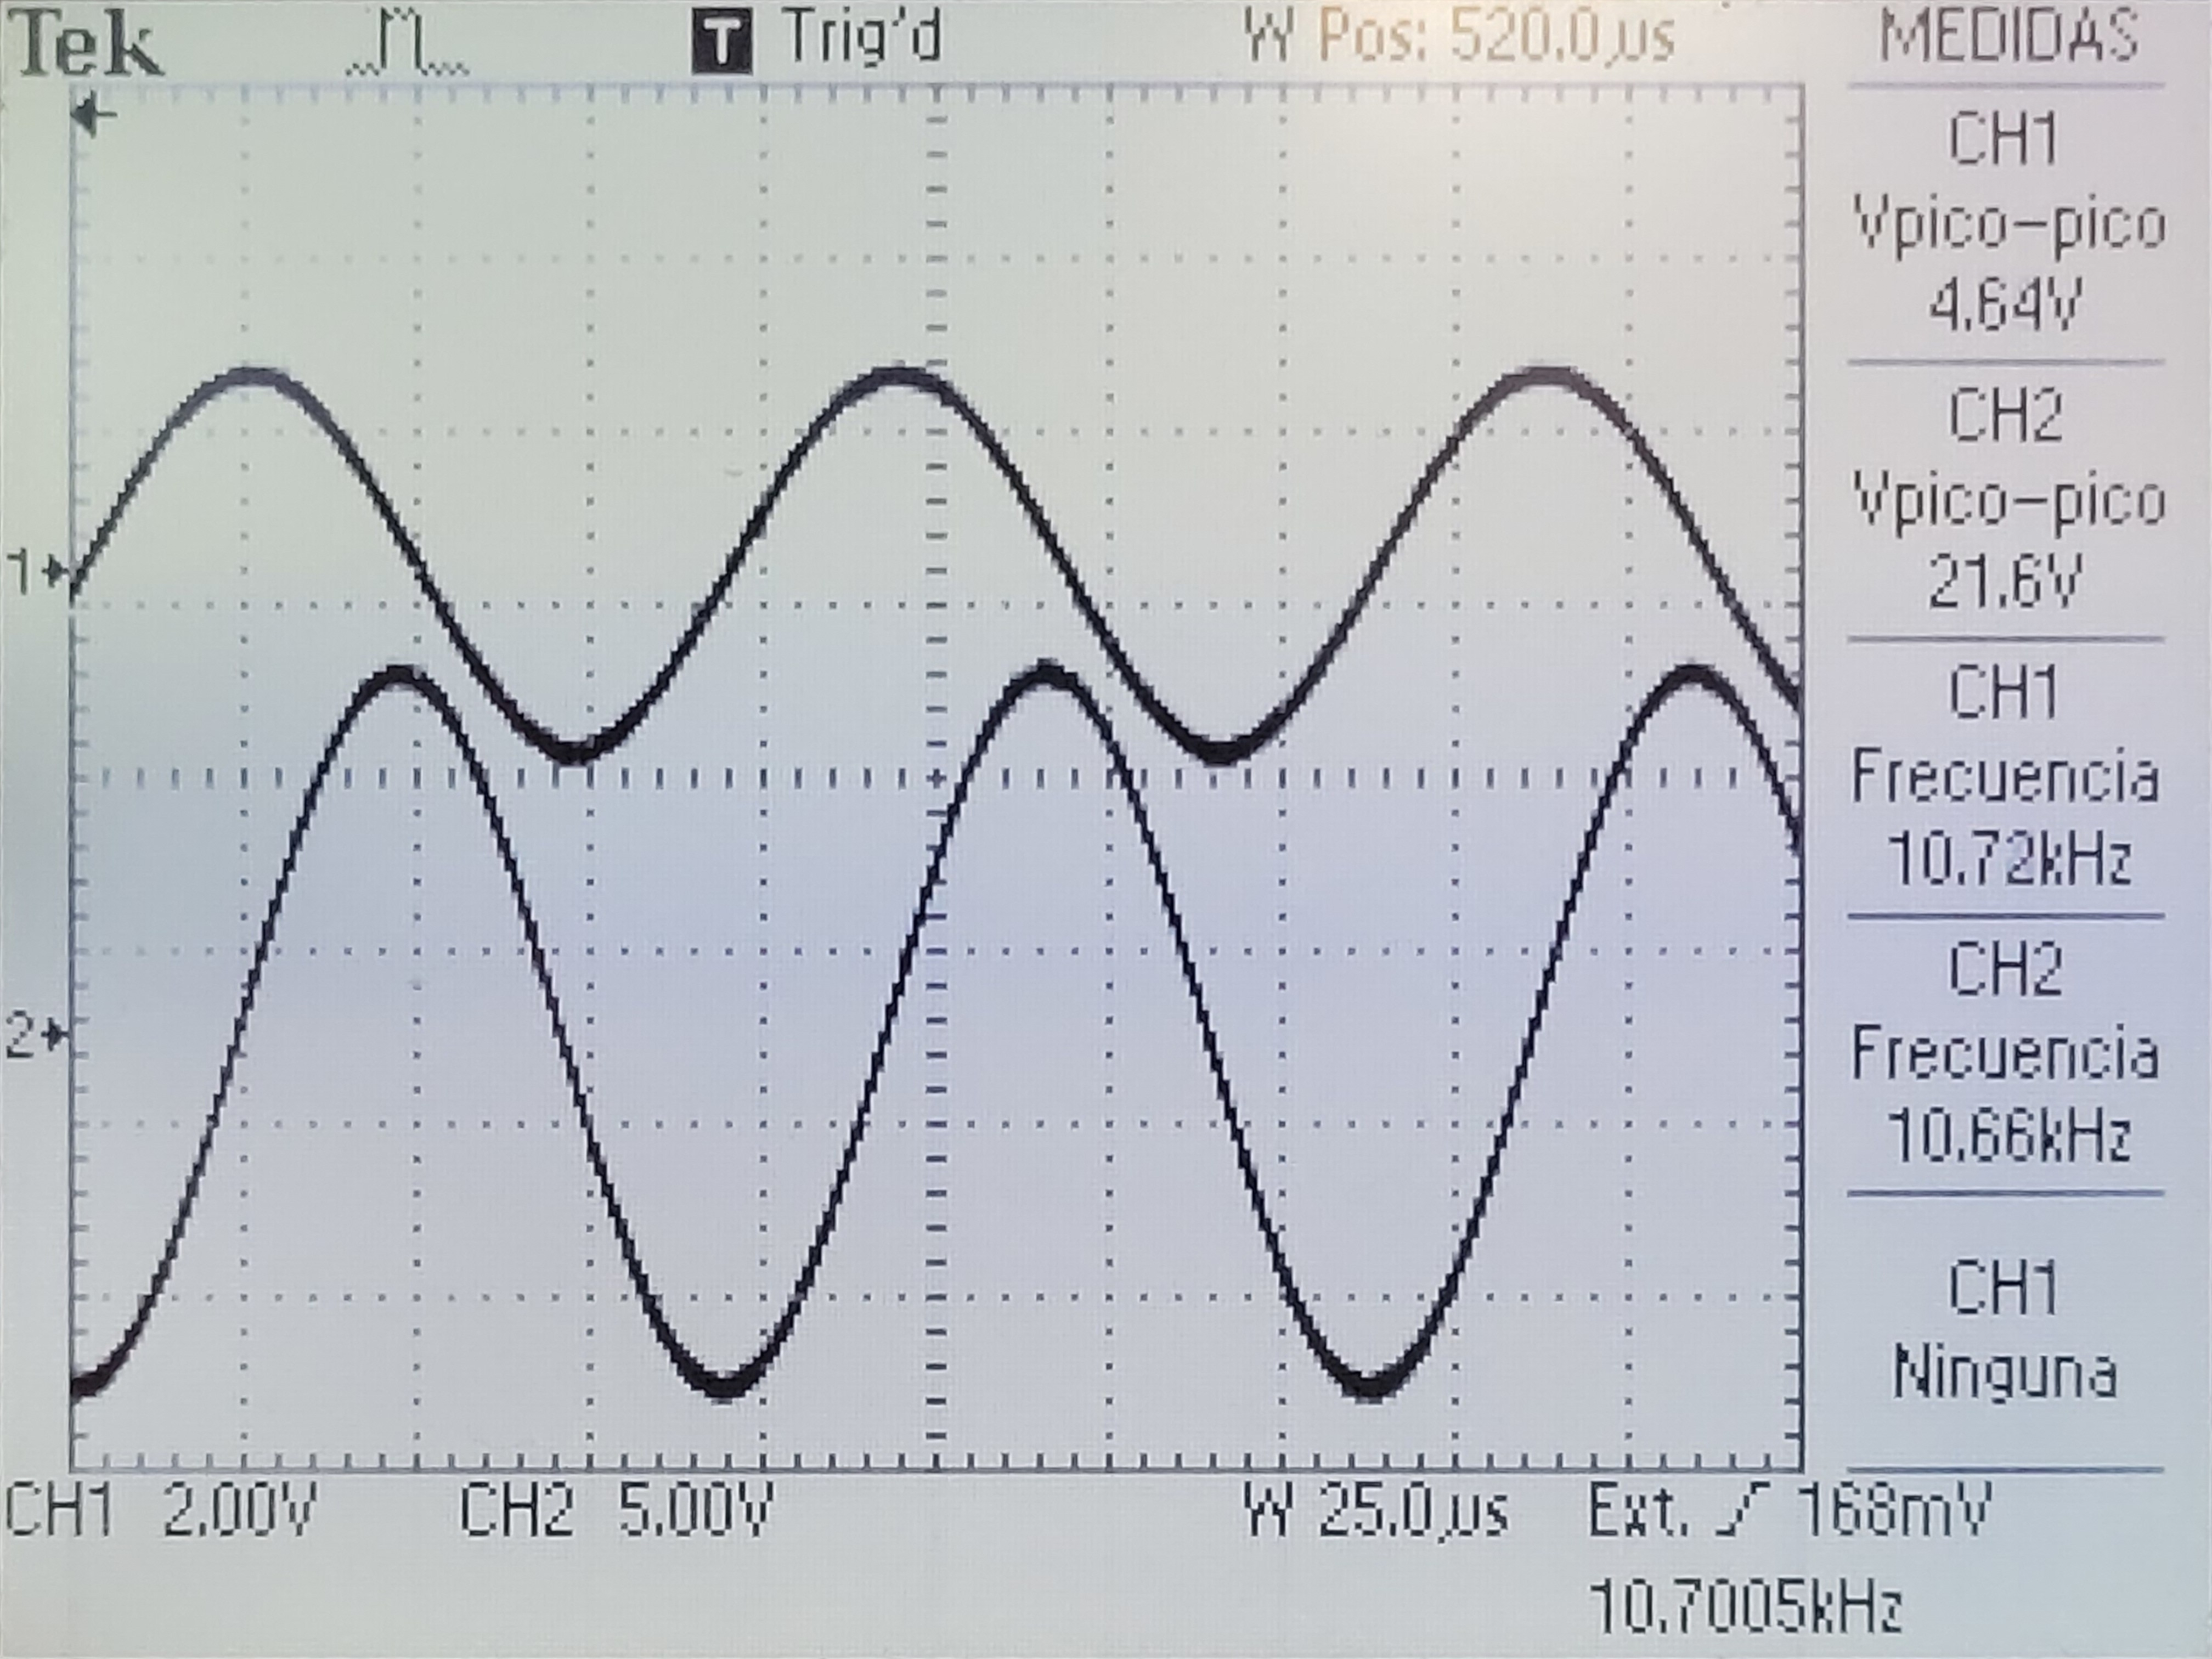
\includegraphics[width=0.65\textwidth]{pictures/osc_fino_f0.jpeg}
    \caption{Resonancia exacta ($f_0 = \qty{10.70}{\kilo\hertz}$).}
    \label{fig.ej1:osc_fino_f0}
\end{figure}

Tal como se evidencia en la captura de la Figura~\ref{fig.ej1:osc_fino_f0}, la resonancia del sistema se alcanzó a:
\begin{equation}
    f_0 = \qty{10.70}{\kilo\hertz} \quad (f_{\text{ext}} = \qty{10.7005}{\kilo\hertz})
    \label{eq.ej1:f0_medida}
\end{equation}
En este punto singular se relevaron los siguientes valores de tensión:
\begin{itemize}
    \item Tensión total aplicada: $e_{\text{tot}} = \qty{4.64}{\volt_{\text{pp}}}$
    \item Tensión en el capacitor: $V_{C,\text{max}} = \qty{21.6}{\volt_{\text{pp}}}$.
\end{itemize}
Nótese que la tensión total $e_{\text{tot}}$ experimenta una disminución desde sus $\qty{5.0}{\volt_{\text{pp}}}$
nominales hasta $\qty{4.64}{\volt_{\text{pp}}}$. Este efecto responde a la ley de Ohm: en resonancia la
impedancia del circuito LC se reduce a su valor mínimo ($Z = R_L$), maximizando la corriente de malla y provocando la
mayor caída de tensión sobre la resistencia de salida del generador y la resistencia de protección ($R_g + r = \qty{97}{\ohm}$).

Asimismo, en la pantalla del osciloscopio se aprecia con nitidez la relación de fase: la tensión en el capacitor se
encuentra retrasada $90^\circ$ respecto a la corriente de malla.

\subsection{Determinación de las Frecuencias de Corte a -3 dB}
Para establecer el ancho de banda y el factor de calidad, calculamos el umbral de tensión correspondiente a la potencia
mitad ($\qty{-3}{\decibel}$ por debajo del máximo):
\begin{equation}
    V_{-3\text{dB}} = \frac{V_{C,\text{max}}}{\sqrt{2}} = \frac{\qty{21.6}{\volt_{\text{pp}}}}{\sqrt{2}} \approx \qty{15.27}{\volt_{\text{pp}}}
    \label{eq.ej1:calculo_umbral}
\end{equation}

\subsubsection{Frecuencia de Corte Inferior ($f_{\text{inf}}$)}
Se realizó un barrido fino en el intervalo comprendido entre $\qty{9000}{\hertz}$ y $\qty{9500}{\hertz}$ con saltos de
$\qty{100}{\hertz}$ en modo manual. En el paso 2 del barrido, correspondiente a $\qty{9100.0}{\hertz}$ , la tensión en
CH2 alcanzó con exactitud el nivel de $\qty{15.2}{\volt_{\text{pp}}}$.

\begin{figure}[!ht]
    \centering
    \begin{subfigure}[t]{0.48\textwidth}
        \centering
        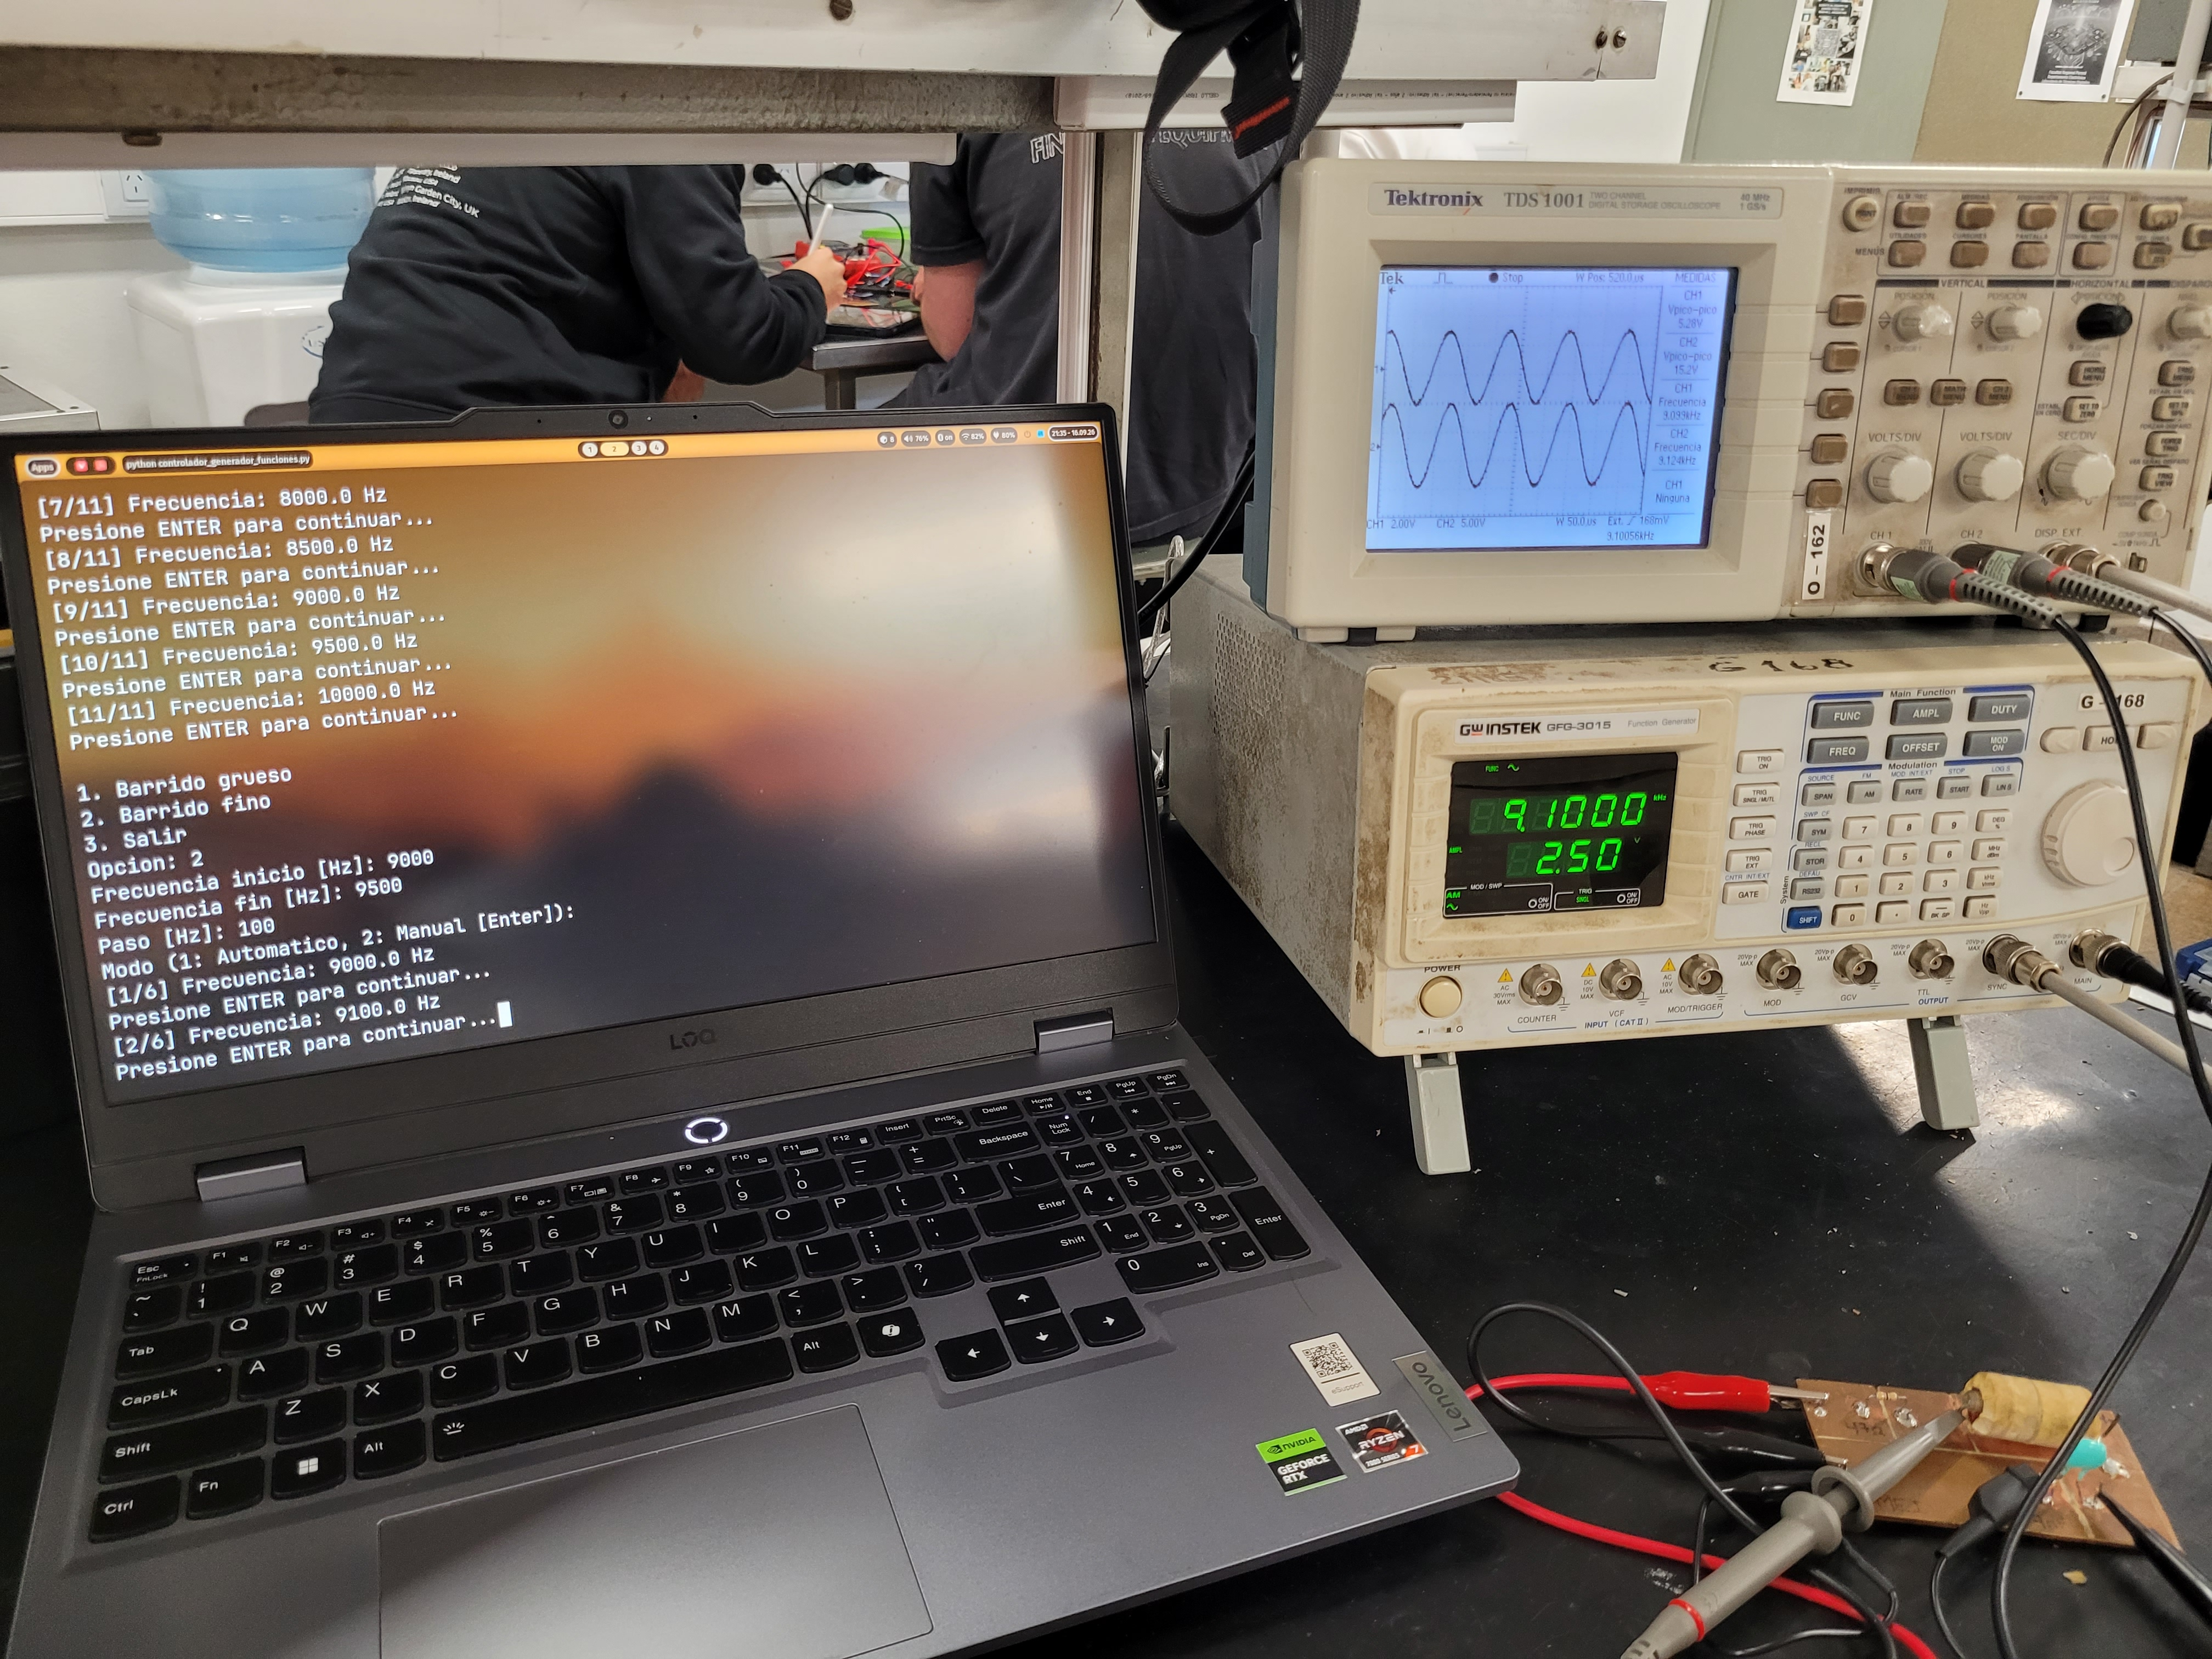
\includegraphics[width=\textwidth]{pictures/setup_fino_finf.jpeg}
        \caption{Paso de barrido en $\qty{9100}{\hertz}$.}
        \label{fig.ej1:setup_fino_finf}
    \end{subfigure}
    \hfill
    \begin{subfigure}[t]{0.48\textwidth}
        \centering
        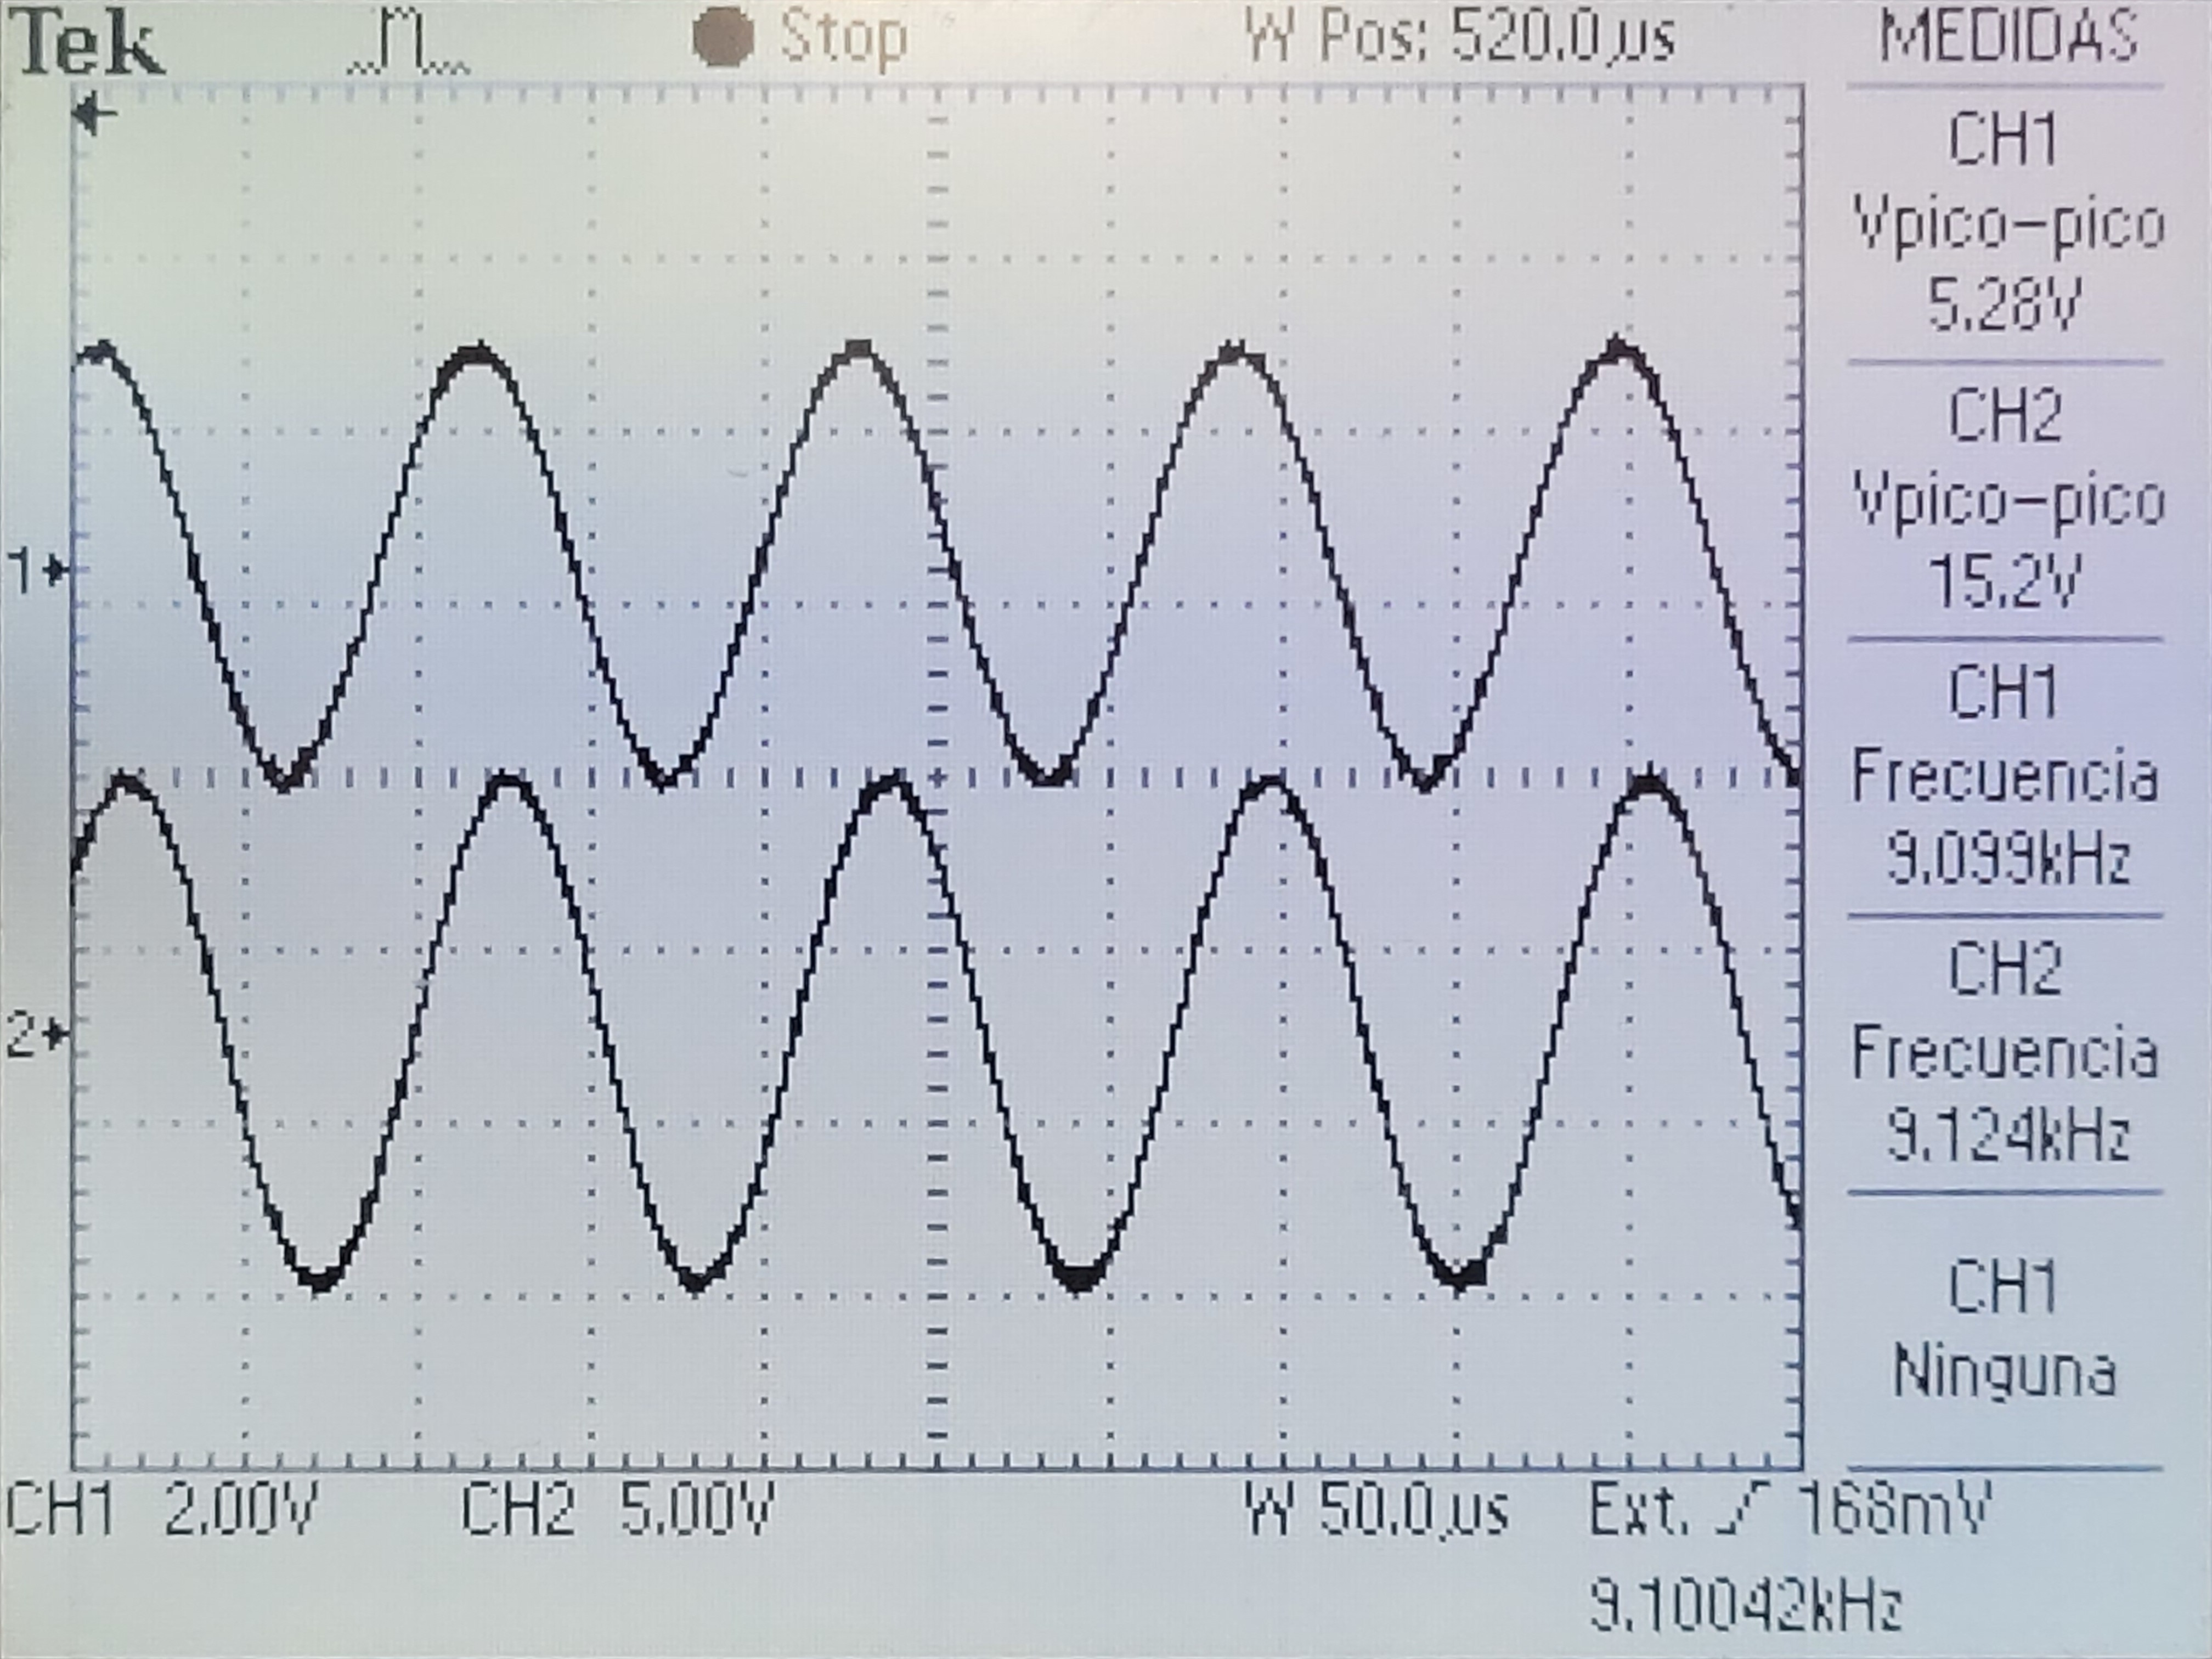
\includegraphics[width=\textwidth]{pictures/osc_fino_finf.jpeg}
        \caption{Formas de onda en $f_{\text{inf}} = \qty{9.10}{\kilo\hertz}$.}
        \label{fig.ej1:osc_fino_finf}
    \end{subfigure}
    \caption{Medición de la frecuencia de corte inferior ($f_{\text{inf}}$) a $\qty{-3}{\decibel}$.}
    \label{fig.ej1:corte_inferior}
\end{figure}

En la Figura~\ref{fig.ej1:corte_inferior} se muestran la consola de control y la pantalla del osciloscopio:
\begin{itemize}
    \item Frecuencia de corte inferior: $f_{\text{inf}} = \qty{9.10}{\kilo\hertz}$.
    \item Tensión en el capacitor (CH2): $V_C = \qty{15.2}{\volt_{\text{pp}}}$.
\end{itemize}

\subsubsection{Frecuencia de Corte Superior ($f_{\text{sup}}$)}
Se realizó un barrido fino ascendente en el rango de $\qty{11900}{\hertz}$ a $\qty{12100}{\hertz}$ con paso de
$\qty{50}{\hertz}$. Al alcanzar el paso 4, correspondiente a una frecuencia de $\qty{12050.0}{\hertz}$, la tensión en el
capacitor se redujo nuevamente a $\qty{15.2}{\volt_{\text{pp}}}$.

\begin{figure}[!ht]
    \centering
    \begin{subfigure}[t]{0.48\textwidth}
        \centering
        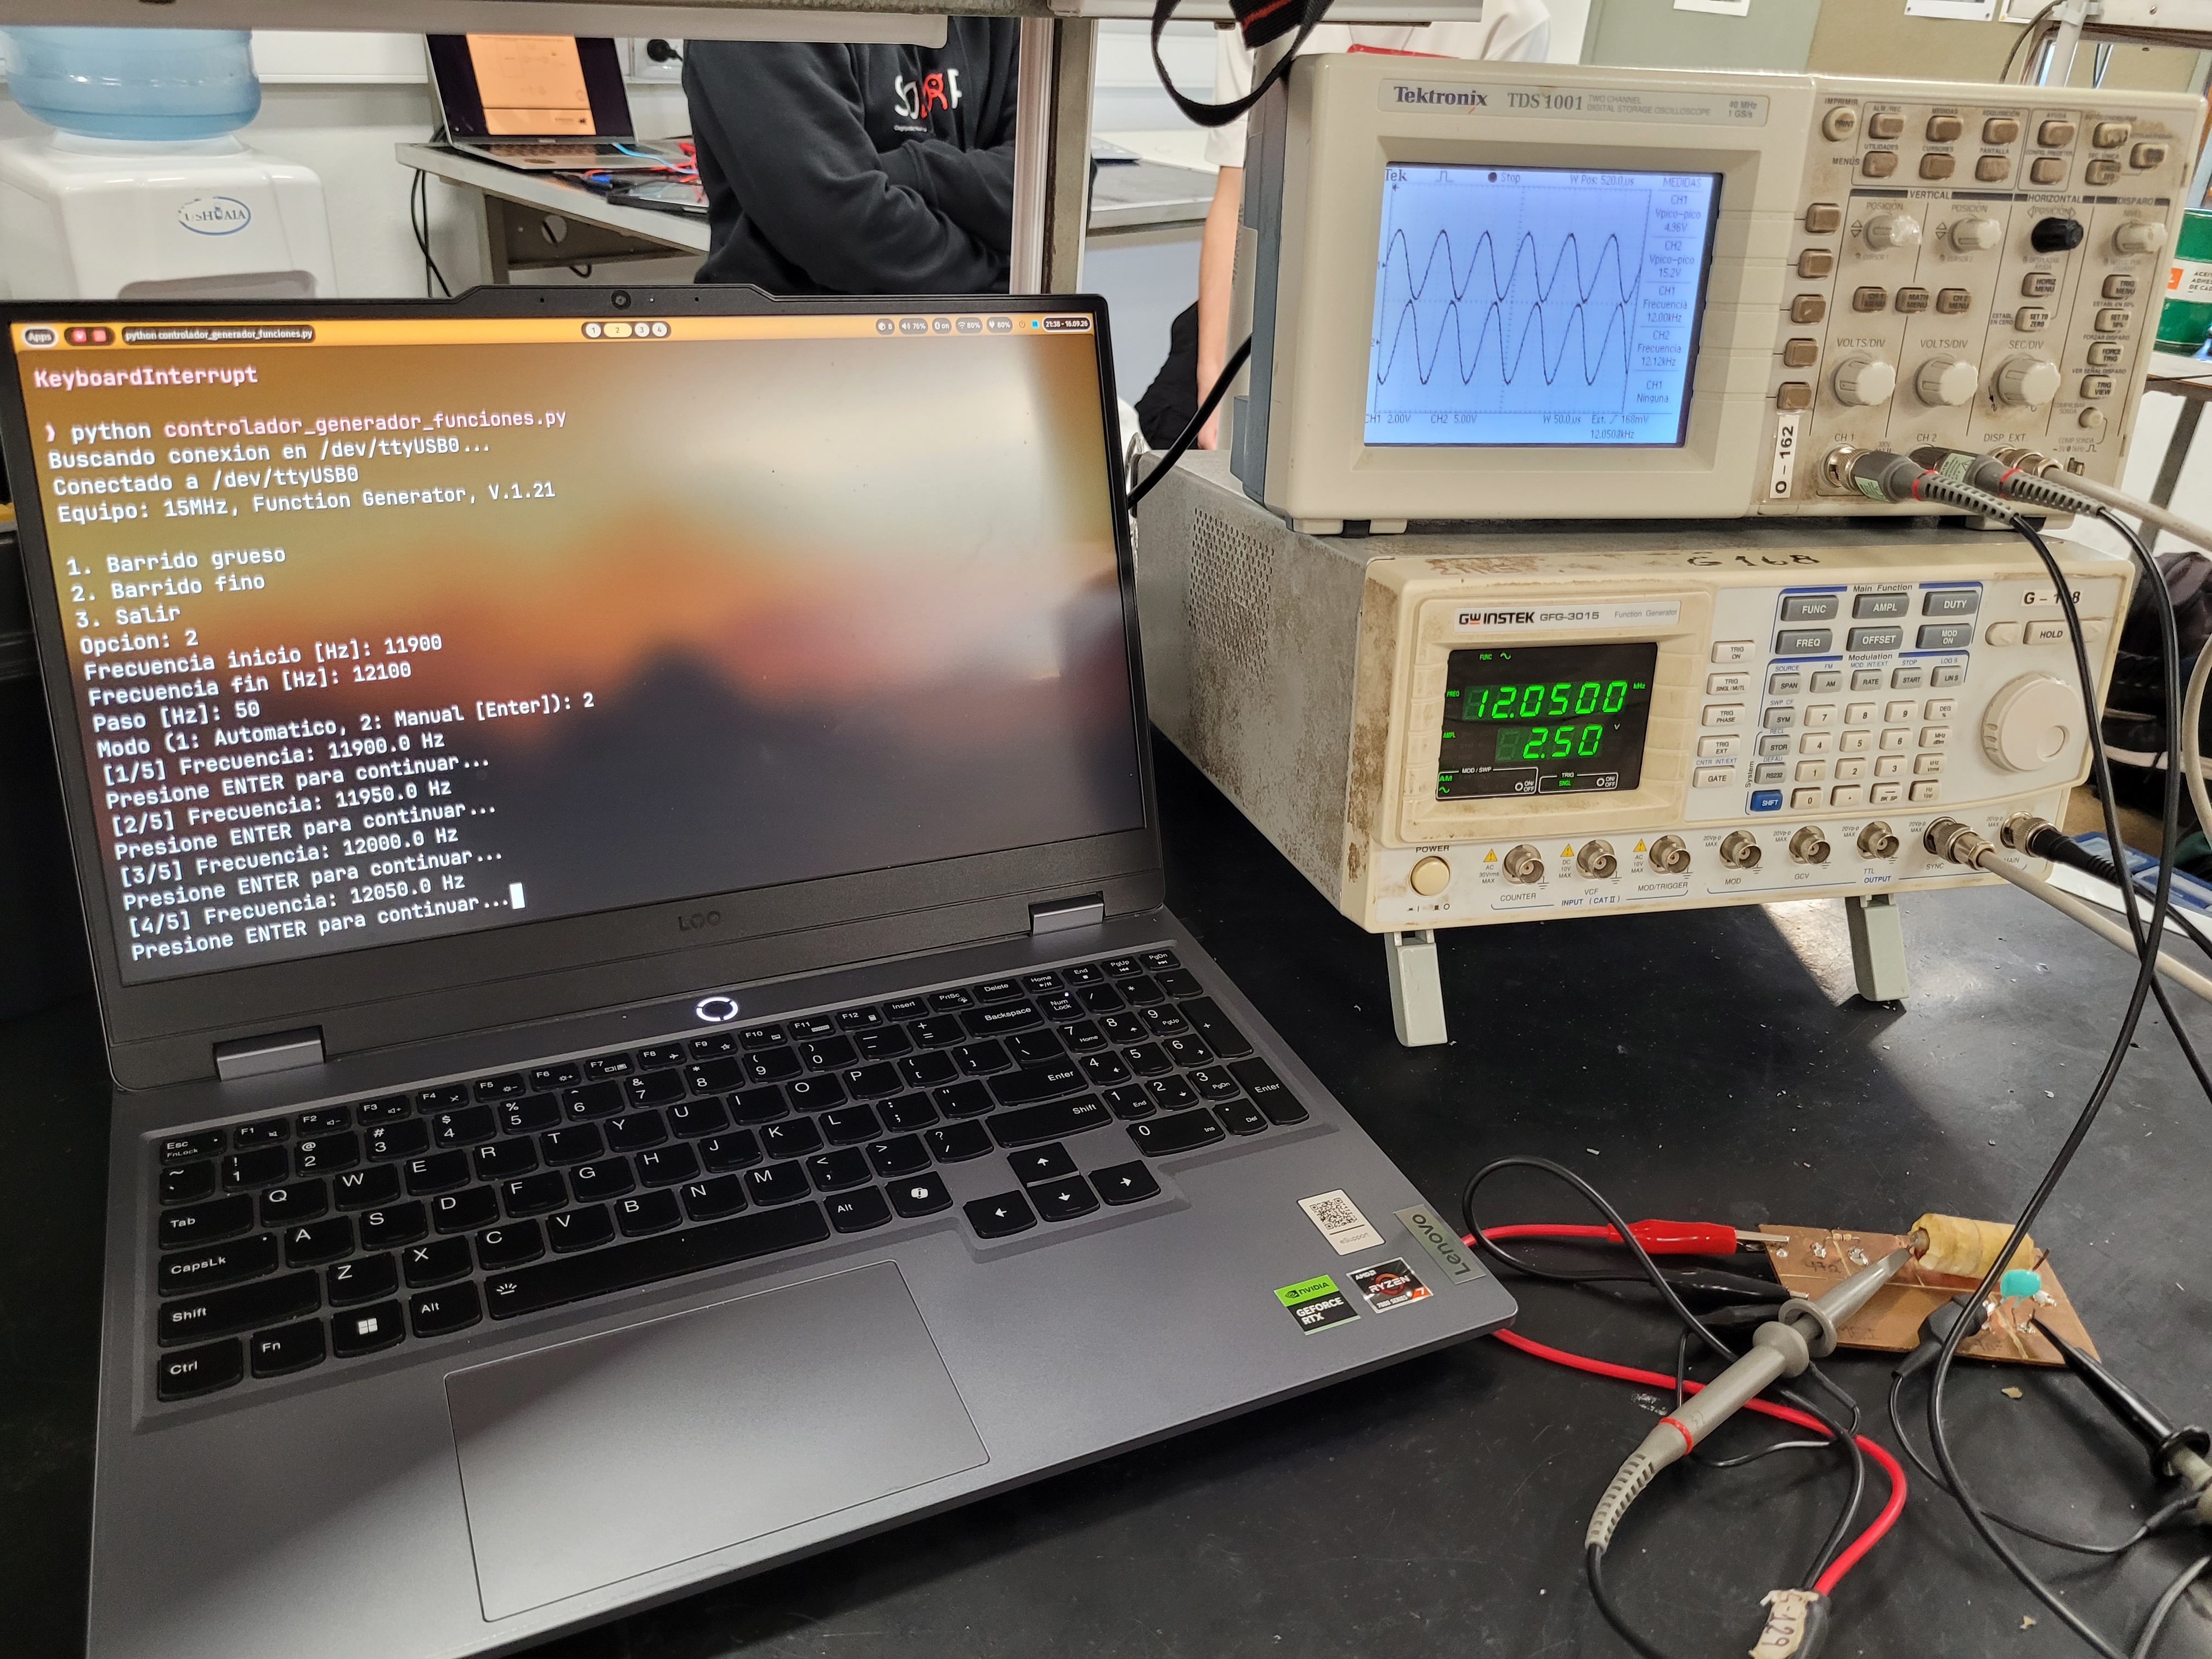
\includegraphics[width=\textwidth]{pictures/setup_fino_fsup.jpeg}
        \caption{Paso de barrido en $\qty{12050}{\hertz}$.}
        \label{fig.ej1:setup_fino_fsup}
    \end{subfigure}
    \hfill
    \begin{subfigure}[t]{0.48\textwidth}
        \centering
        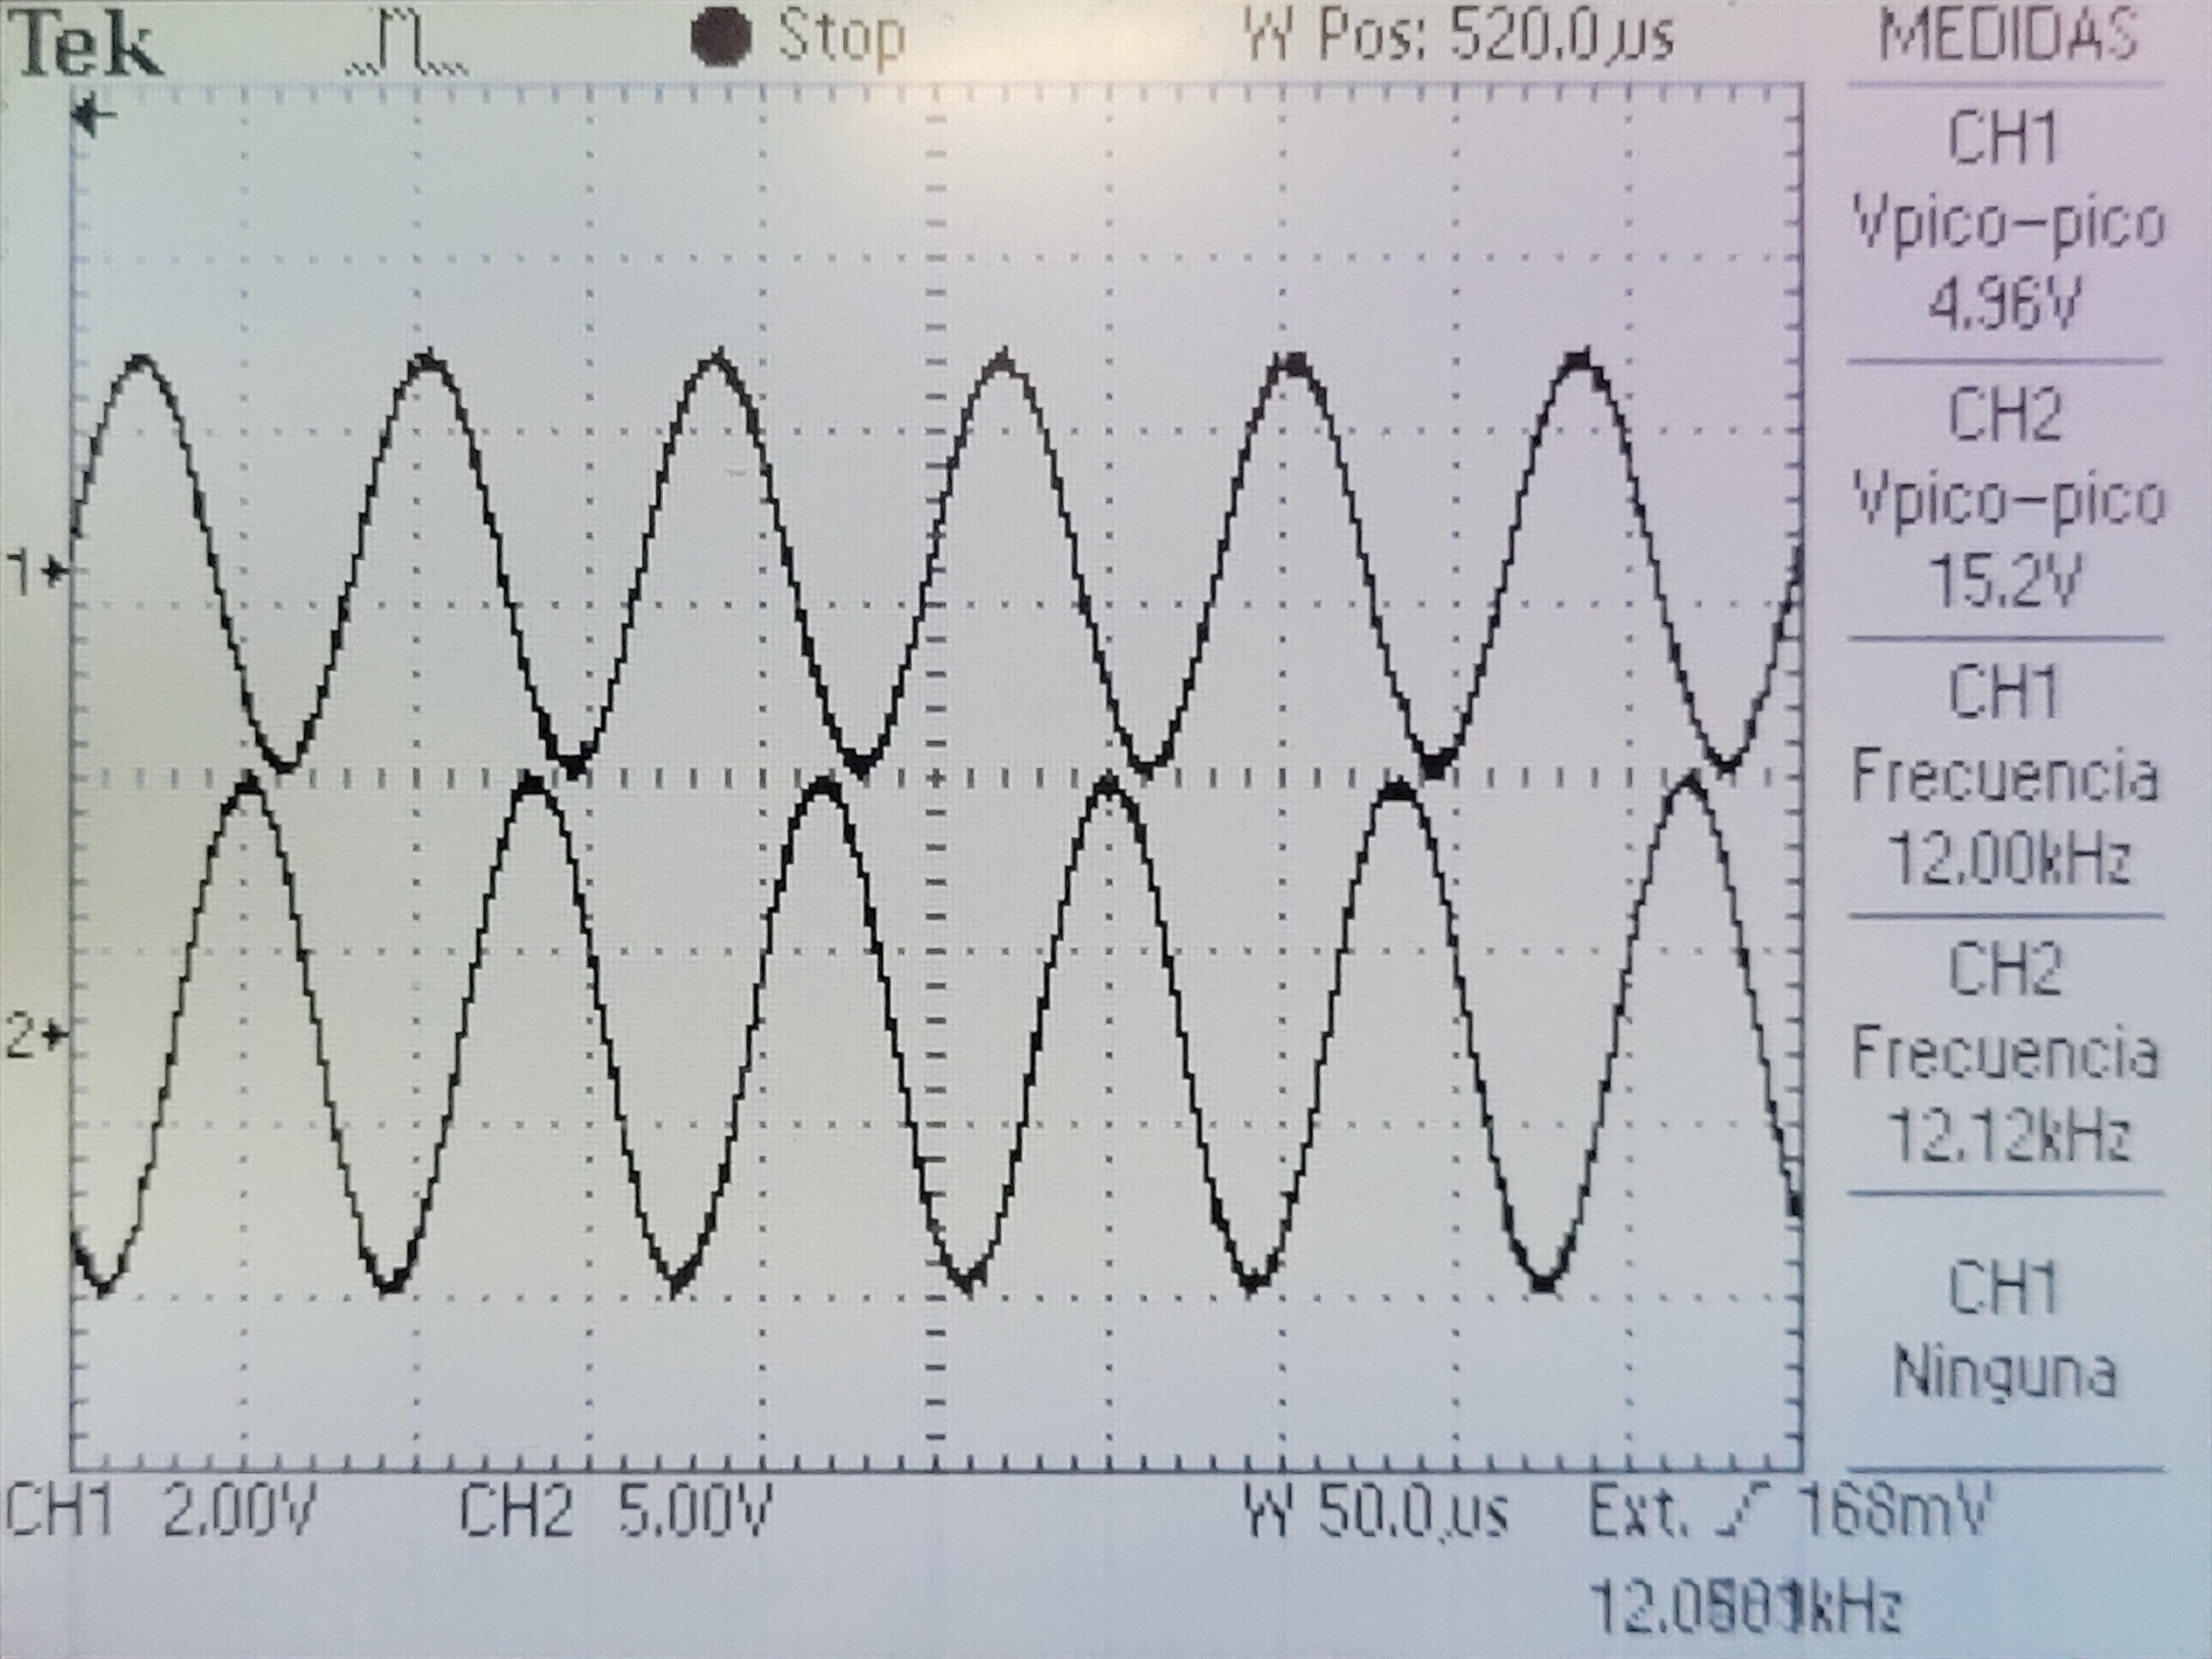
\includegraphics[width=\textwidth]{pictures/osc_fino_fsup.jpeg}
        \caption{Formas de onda en $f_{\text{sup}} = \qty{12.05}{\kilo\hertz}$.}
        \label{fig.ej1:osc_fino_fsup}
    \end{subfigure}
    \caption{Medición de la frecuencia de corte superior ($f_{\text{sup}}$) a $\qty{-3}{\decibel}$.}
    \label{fig.ej1:corte_superior}
\end{figure}

En la Figura~\ref{fig.ej1:corte_superior} se documenta este punto operativo:
\begin{itemize}
    \item Frecuencia de corte superior: $f_{\text{sup}} = \qty{12.05}{\kilo\hertz}$.
    \item Tensión en el capacitor (CH2): $V_C = \qty{15.2}{\volt_{\text{pp}}}$.
\end{itemize}

\section{Cálculo y Análisis del Factor de Calidad (Q)}

Tomando como referencia la tensión total efectivamente aplicada en bornes de la rama resonante ($e_{\text{tot}}$):
\begin{equation}
    Q_v = \frac{V_C(f_0)}{e_{\text{tot}}(f_0)} = \frac{\qty{21.6}{\volt_{\text{pp}}}}{\qty{4.64}{\volt_{\text{pp}}}} = 4.655 \approx 4.66
    \label{eq.ej1:qv_calc}
\end{equation}

\subsection{Contraste con los Valores Nominales}
Los componentes discretos montados en la placa presentan los siguientes valores nominales grabados:
\begin{itemize}
    \item Inductancia nominal: $L = \qty{30}{\milli\henry}$.
    \item Capacitancia nominal: $C = \qty{7}{\nano\farad}$.
\end{itemize}
Calculamos la frecuencia de resonancia teórica mediante la siguiente ecuación:
\begin{equation}
    f_0^{\text{teo}} = \frac{1}{2 \pi \sqrt{L \cdot C}} = \frac{1}{2 \pi \sqrt{(\qty{30e-3}{\henry}) \cdot (\qty{7e-9}{\farad})}} \approx \qty{10.98}{\kilo\hertz}
    \label{eq.ej1:fteo_calc}
\end{equation}
El desvío relativo respecto al valor experimental ($f_0 = \qty{10.70}{\kilo\hertz}$) resulta de apenas:
\begin{equation}
    \varepsilon_r = \frac{|f_0^{\text{med}} - f_0^{\text{teo}}|}{f_0^{\text{teo}}} \times 100\% = \frac{|\qty{10.70}{\kilo\hertz} - \qty{10.98}{\kilo\hertz}|}{\qty{10.98}{\kilo\hertz}} \times 100\% = 2.55\%
    \label{eq.ej1:error_fres}
\end{equation}
Esta concordancia del $2.55\%$ es excelente y se ubica holgadamente dentro del margen de tolerancia constructiva de
capacitores comerciales ($\pm 5\%$ a $\pm 10\%$) e inductores bobinados sobre carrete ($\pm 10\%$).

\section{Validación Espectral mediante Modo FFT y Persistencia Infinita}
Empleamos la Transformada Rápida de Fourier (FFT) del osciloscopio para registrar y validar el comportamiento del filtro
resonante en el dominio de la frecuencia.

\begin{figure}[!ht]
    \centering
    \begin{subfigure}[t]{0.48\textwidth}
        \centering
        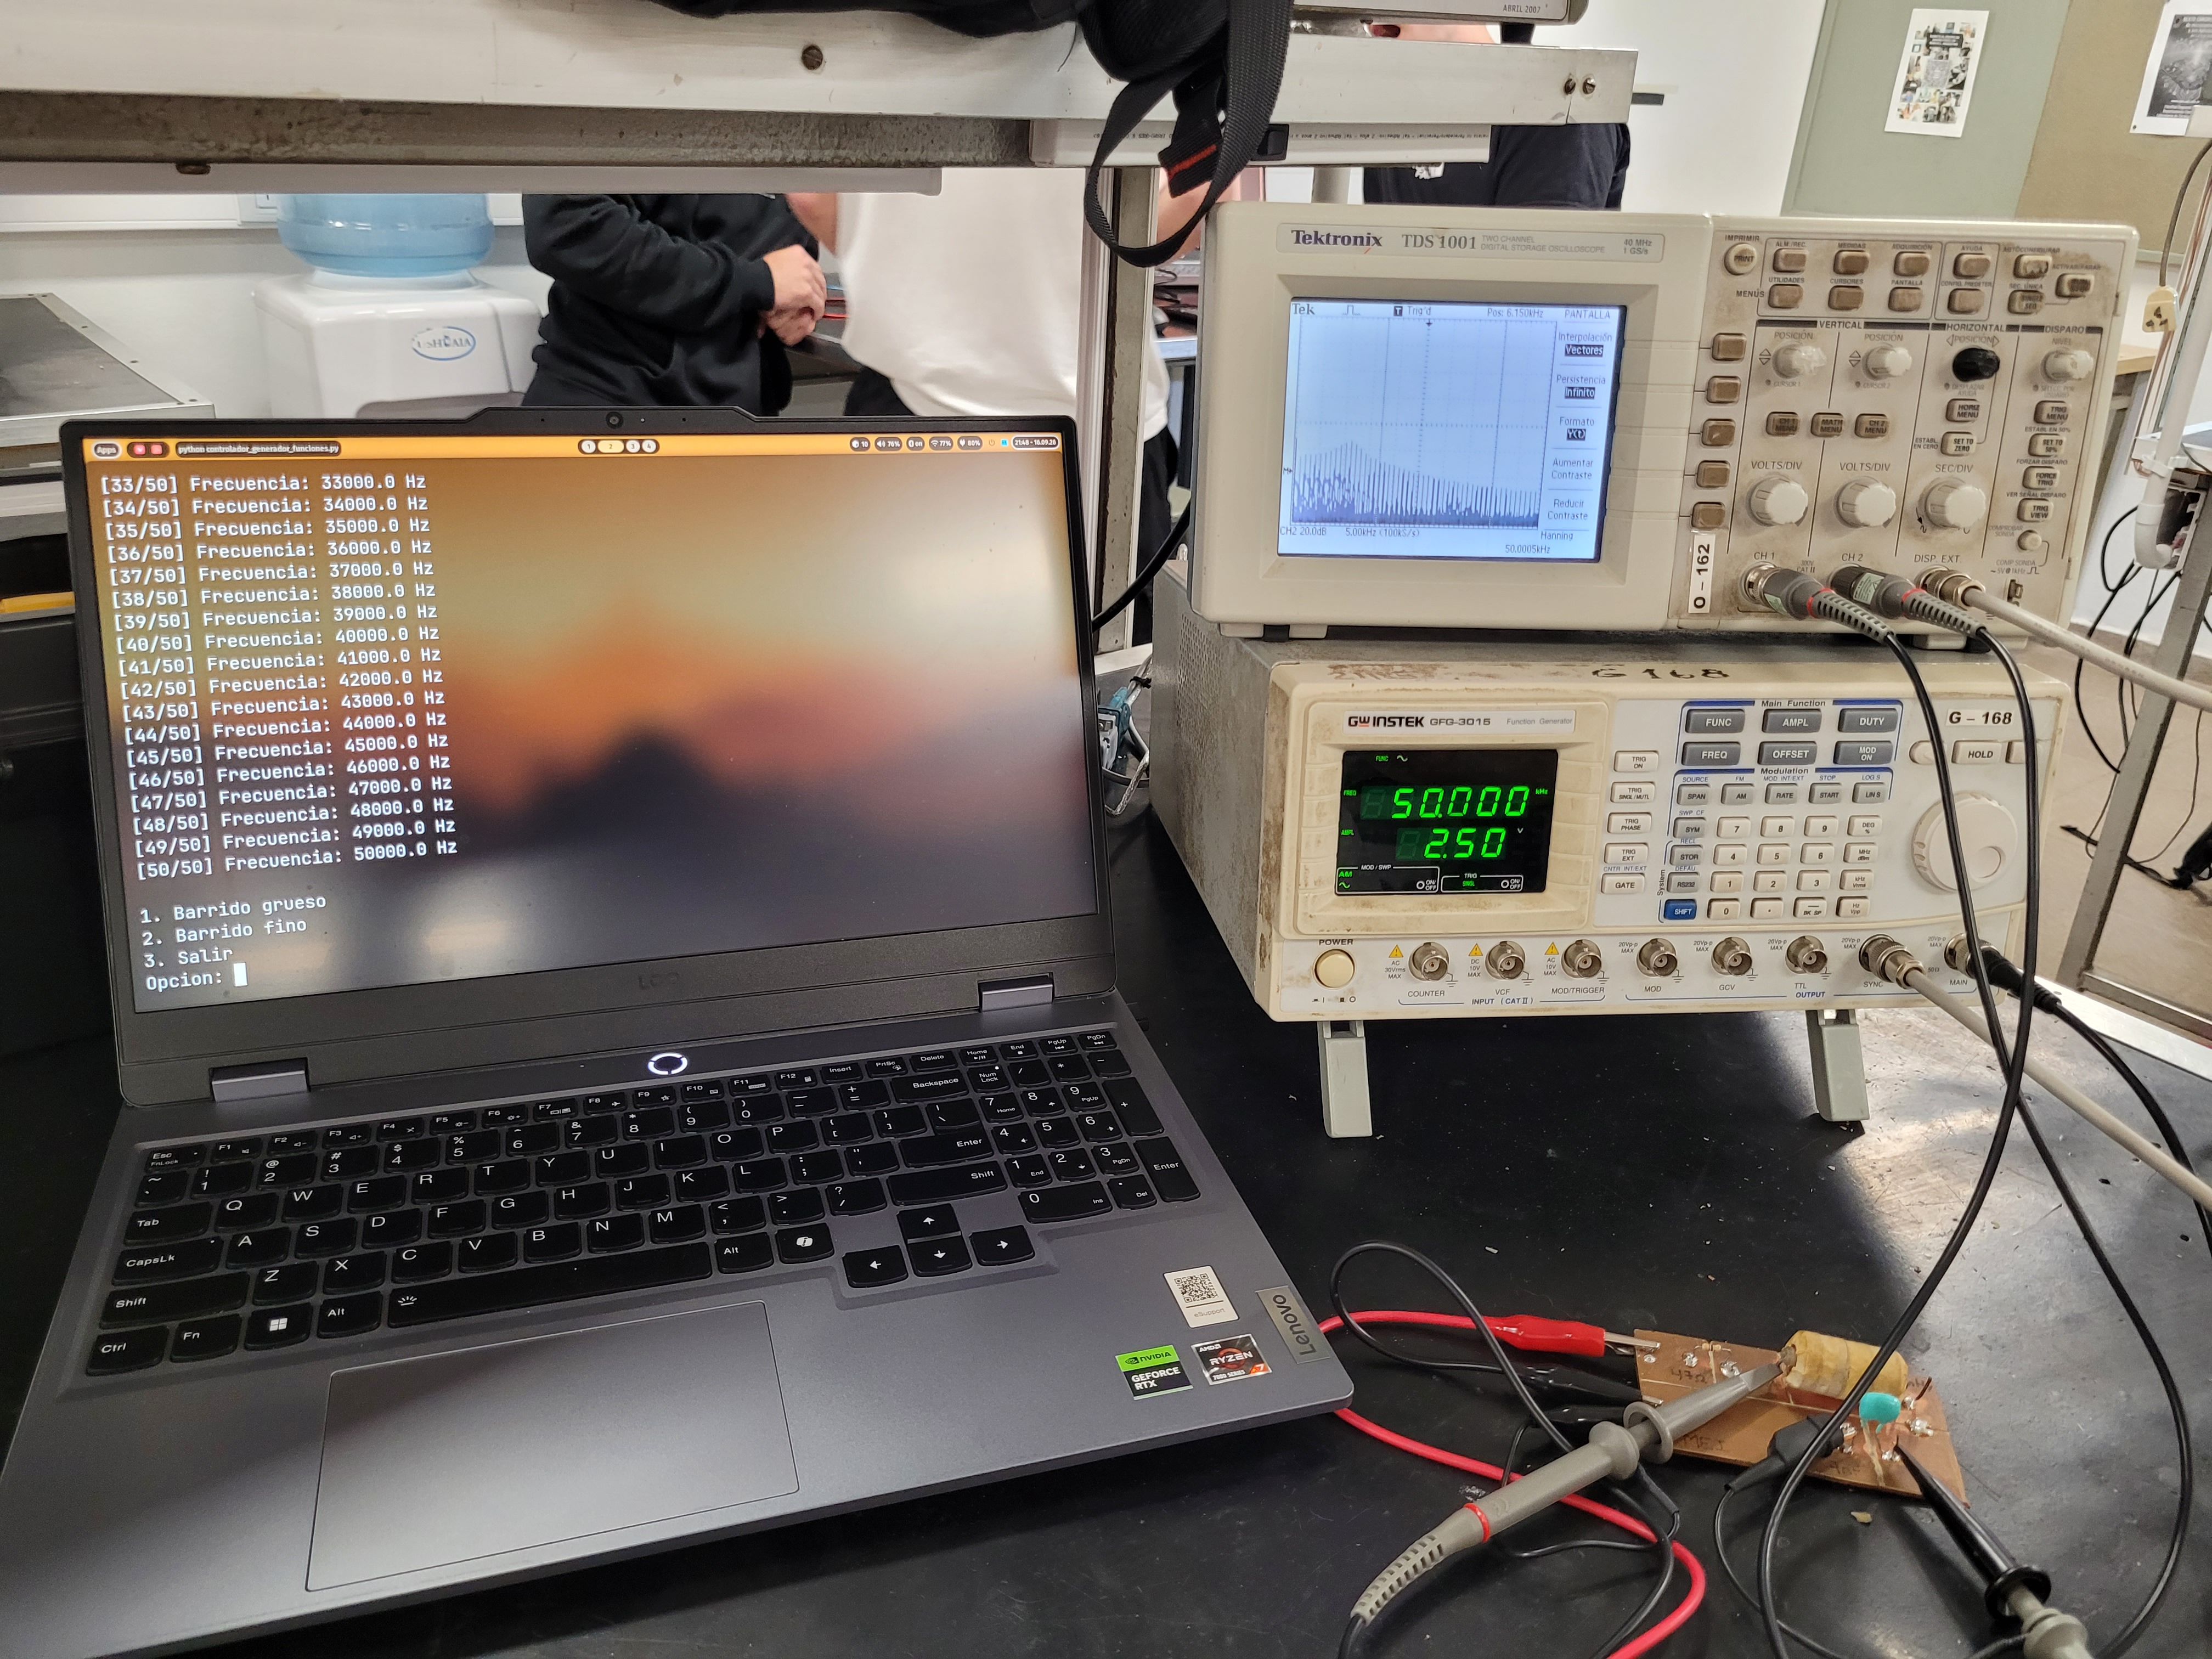
\includegraphics[width=\textwidth]{pictures/setup_fft_barrido_auto_largo.jpeg}
        \caption{Barrido amplio finalizando en paso 50.}
        \label{fig.ej1:setup_fft_largo}
    \end{subfigure}
    \hfill
    \begin{subfigure}[t]{0.48\textwidth}
        \centering
        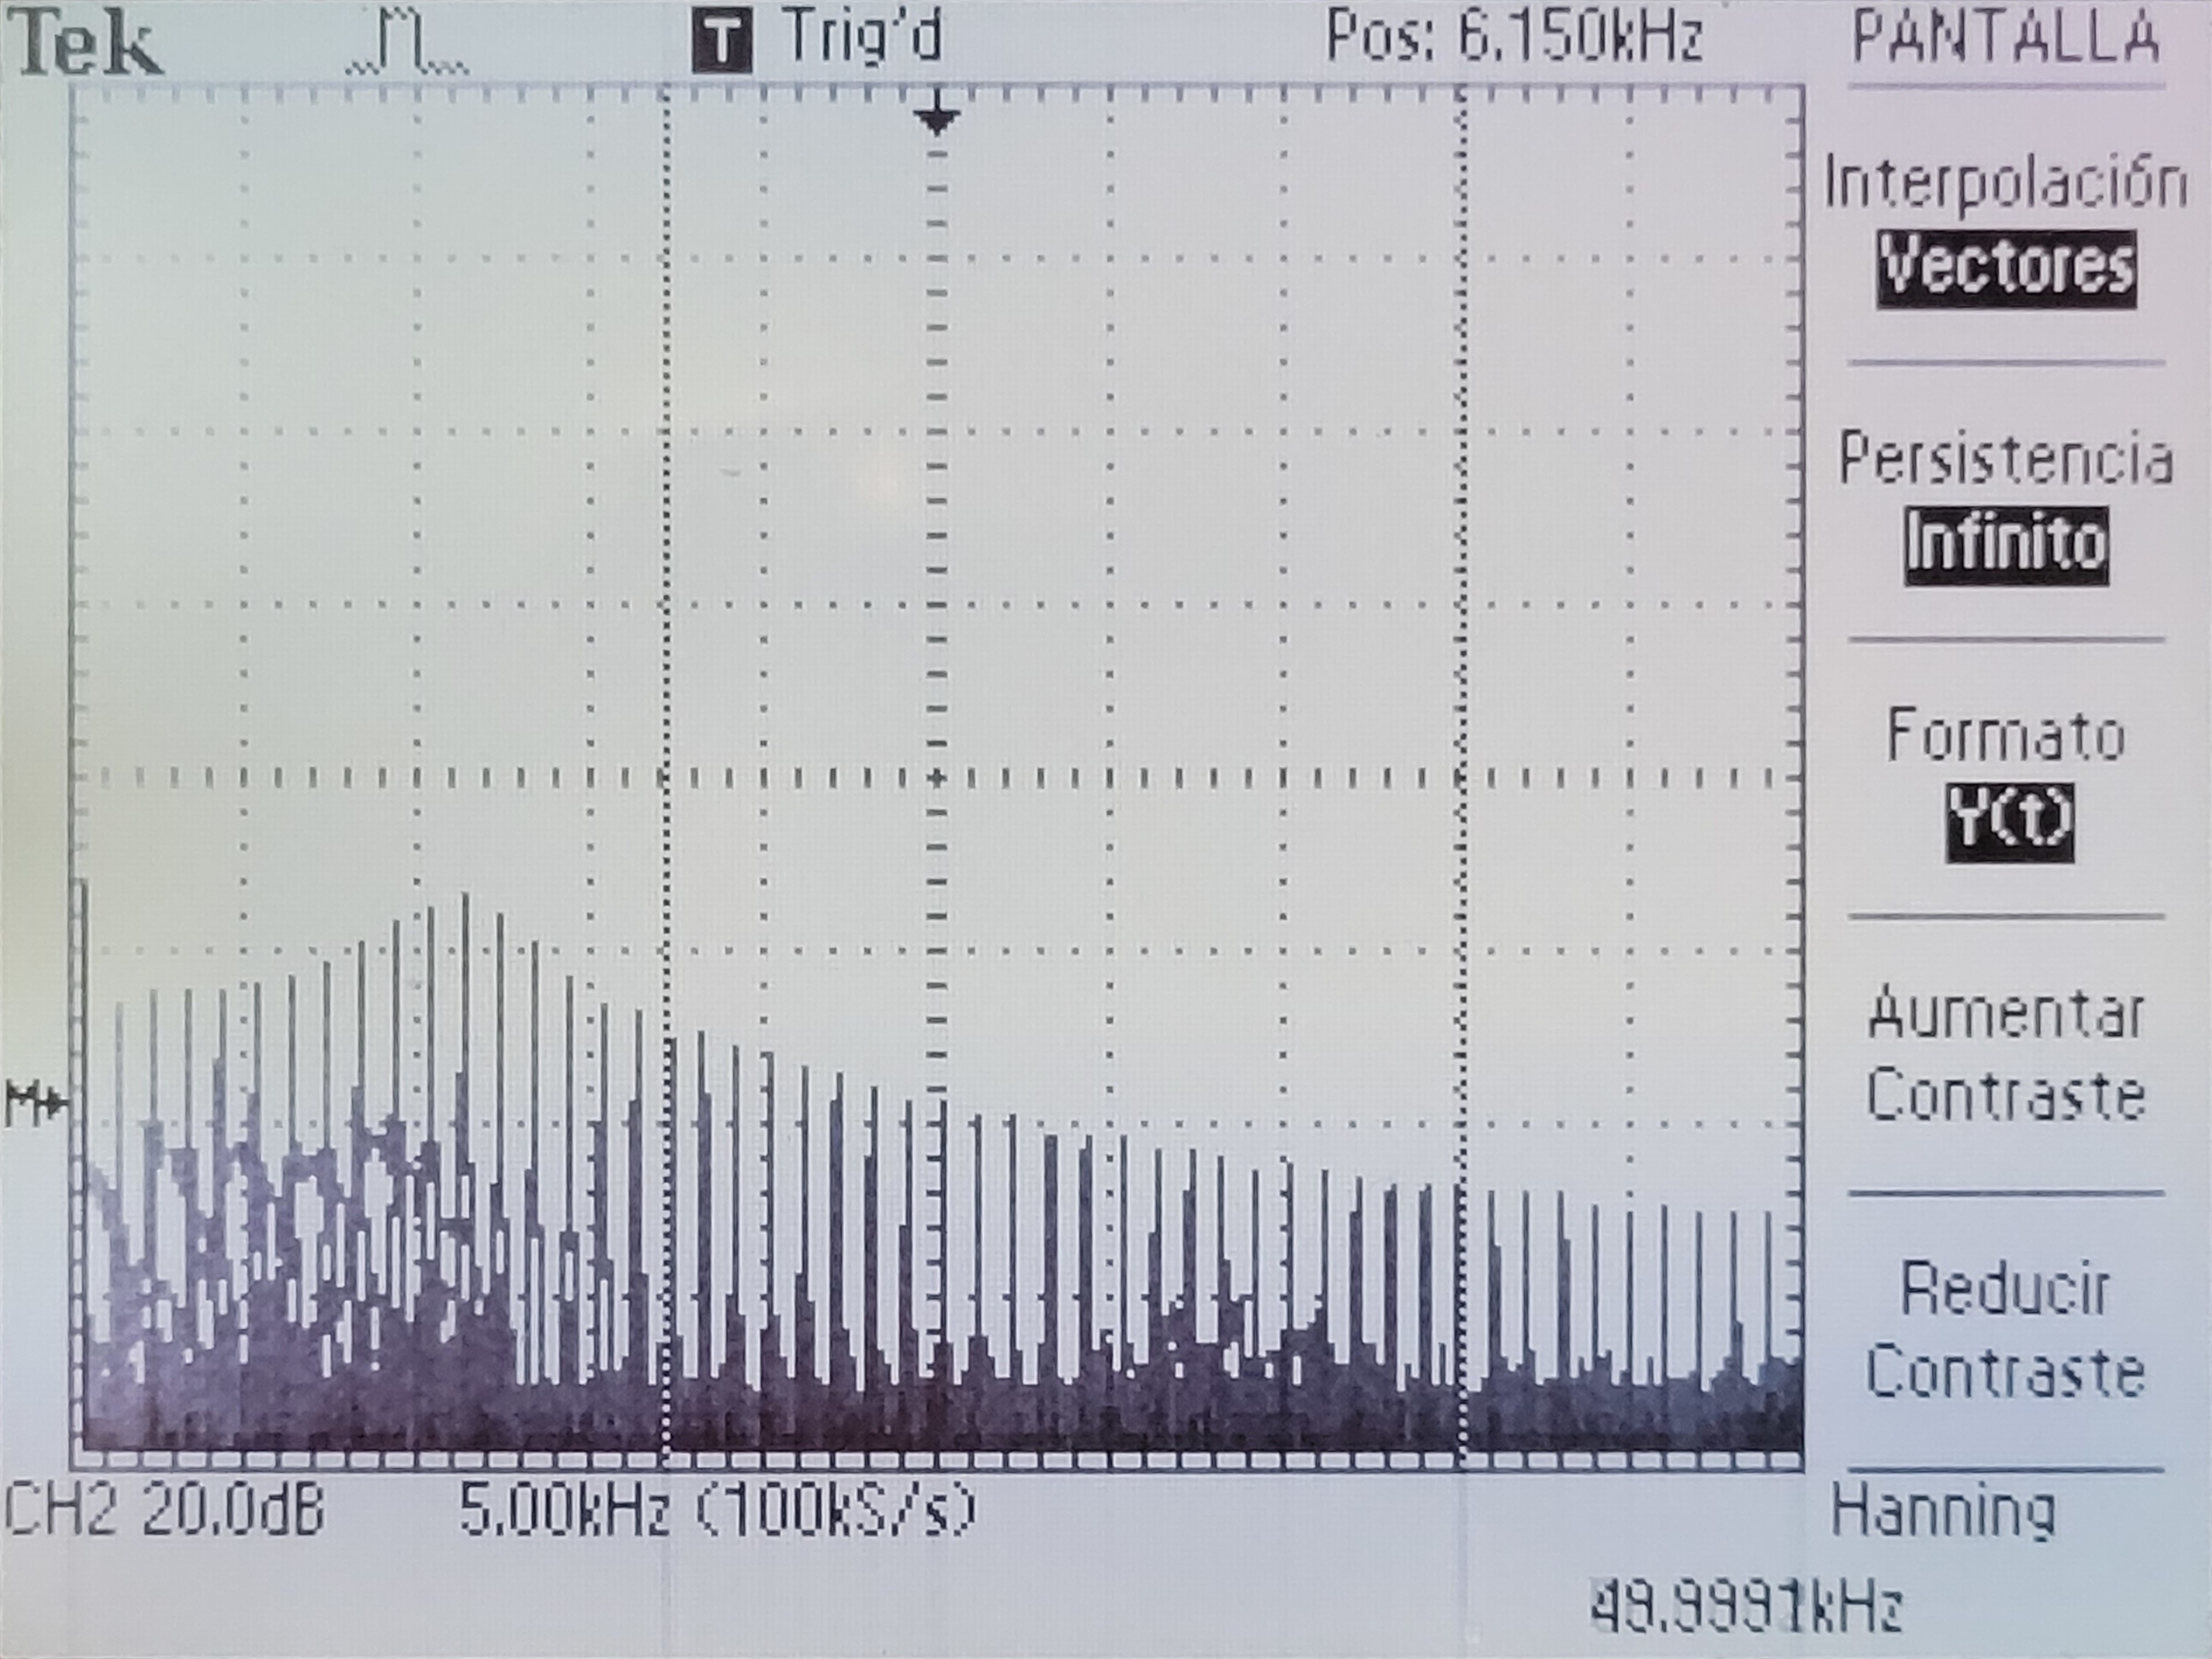
\includegraphics[width=\textwidth]{pictures/osc_fft_barrido_auto_largo.jpeg}
        \caption{Curva envolvente acumulada con persistencia infinita.}
        \label{fig.ej1:osc_fft_largo}
    \end{subfigure}
    \caption{Reconstrucción de la respuesta en frecuencia mediante barrido amplio.}
    \label{fig.ej1:fft_largo}
\end{figure}


El script ejecutó una secuencia automática de 50 pasos cubriendo desde $\qty{1.0}{\kilo\hertz}$ hasta
$\qty{50.0}{\kilo\hertz}$ en saltos de $\qty{1.0}{\kilo\hertz}$. Tal como se observa en la
Figura~\ref{fig.ej1:fft_largo}, se observa la curva caracteristica de amplitud-frecuencia de un filtro pasa-banda con un
circuito RLC. Se observa el rápido crecimiento inicial a frecuencias bajas, el pico resonante en $\sim
\qty{10.7}{\kilo\hertz}$ y la pendiente asintótica de atenuación en alta frecuencia, verificando experimentalmente la
correlación total entre las mediciones en el dominio temporal y el análisis espectral.

\begin{figure}[!ht]
    \centering
    \begin{subfigure}[t]{0.48\textwidth}
        \centering
        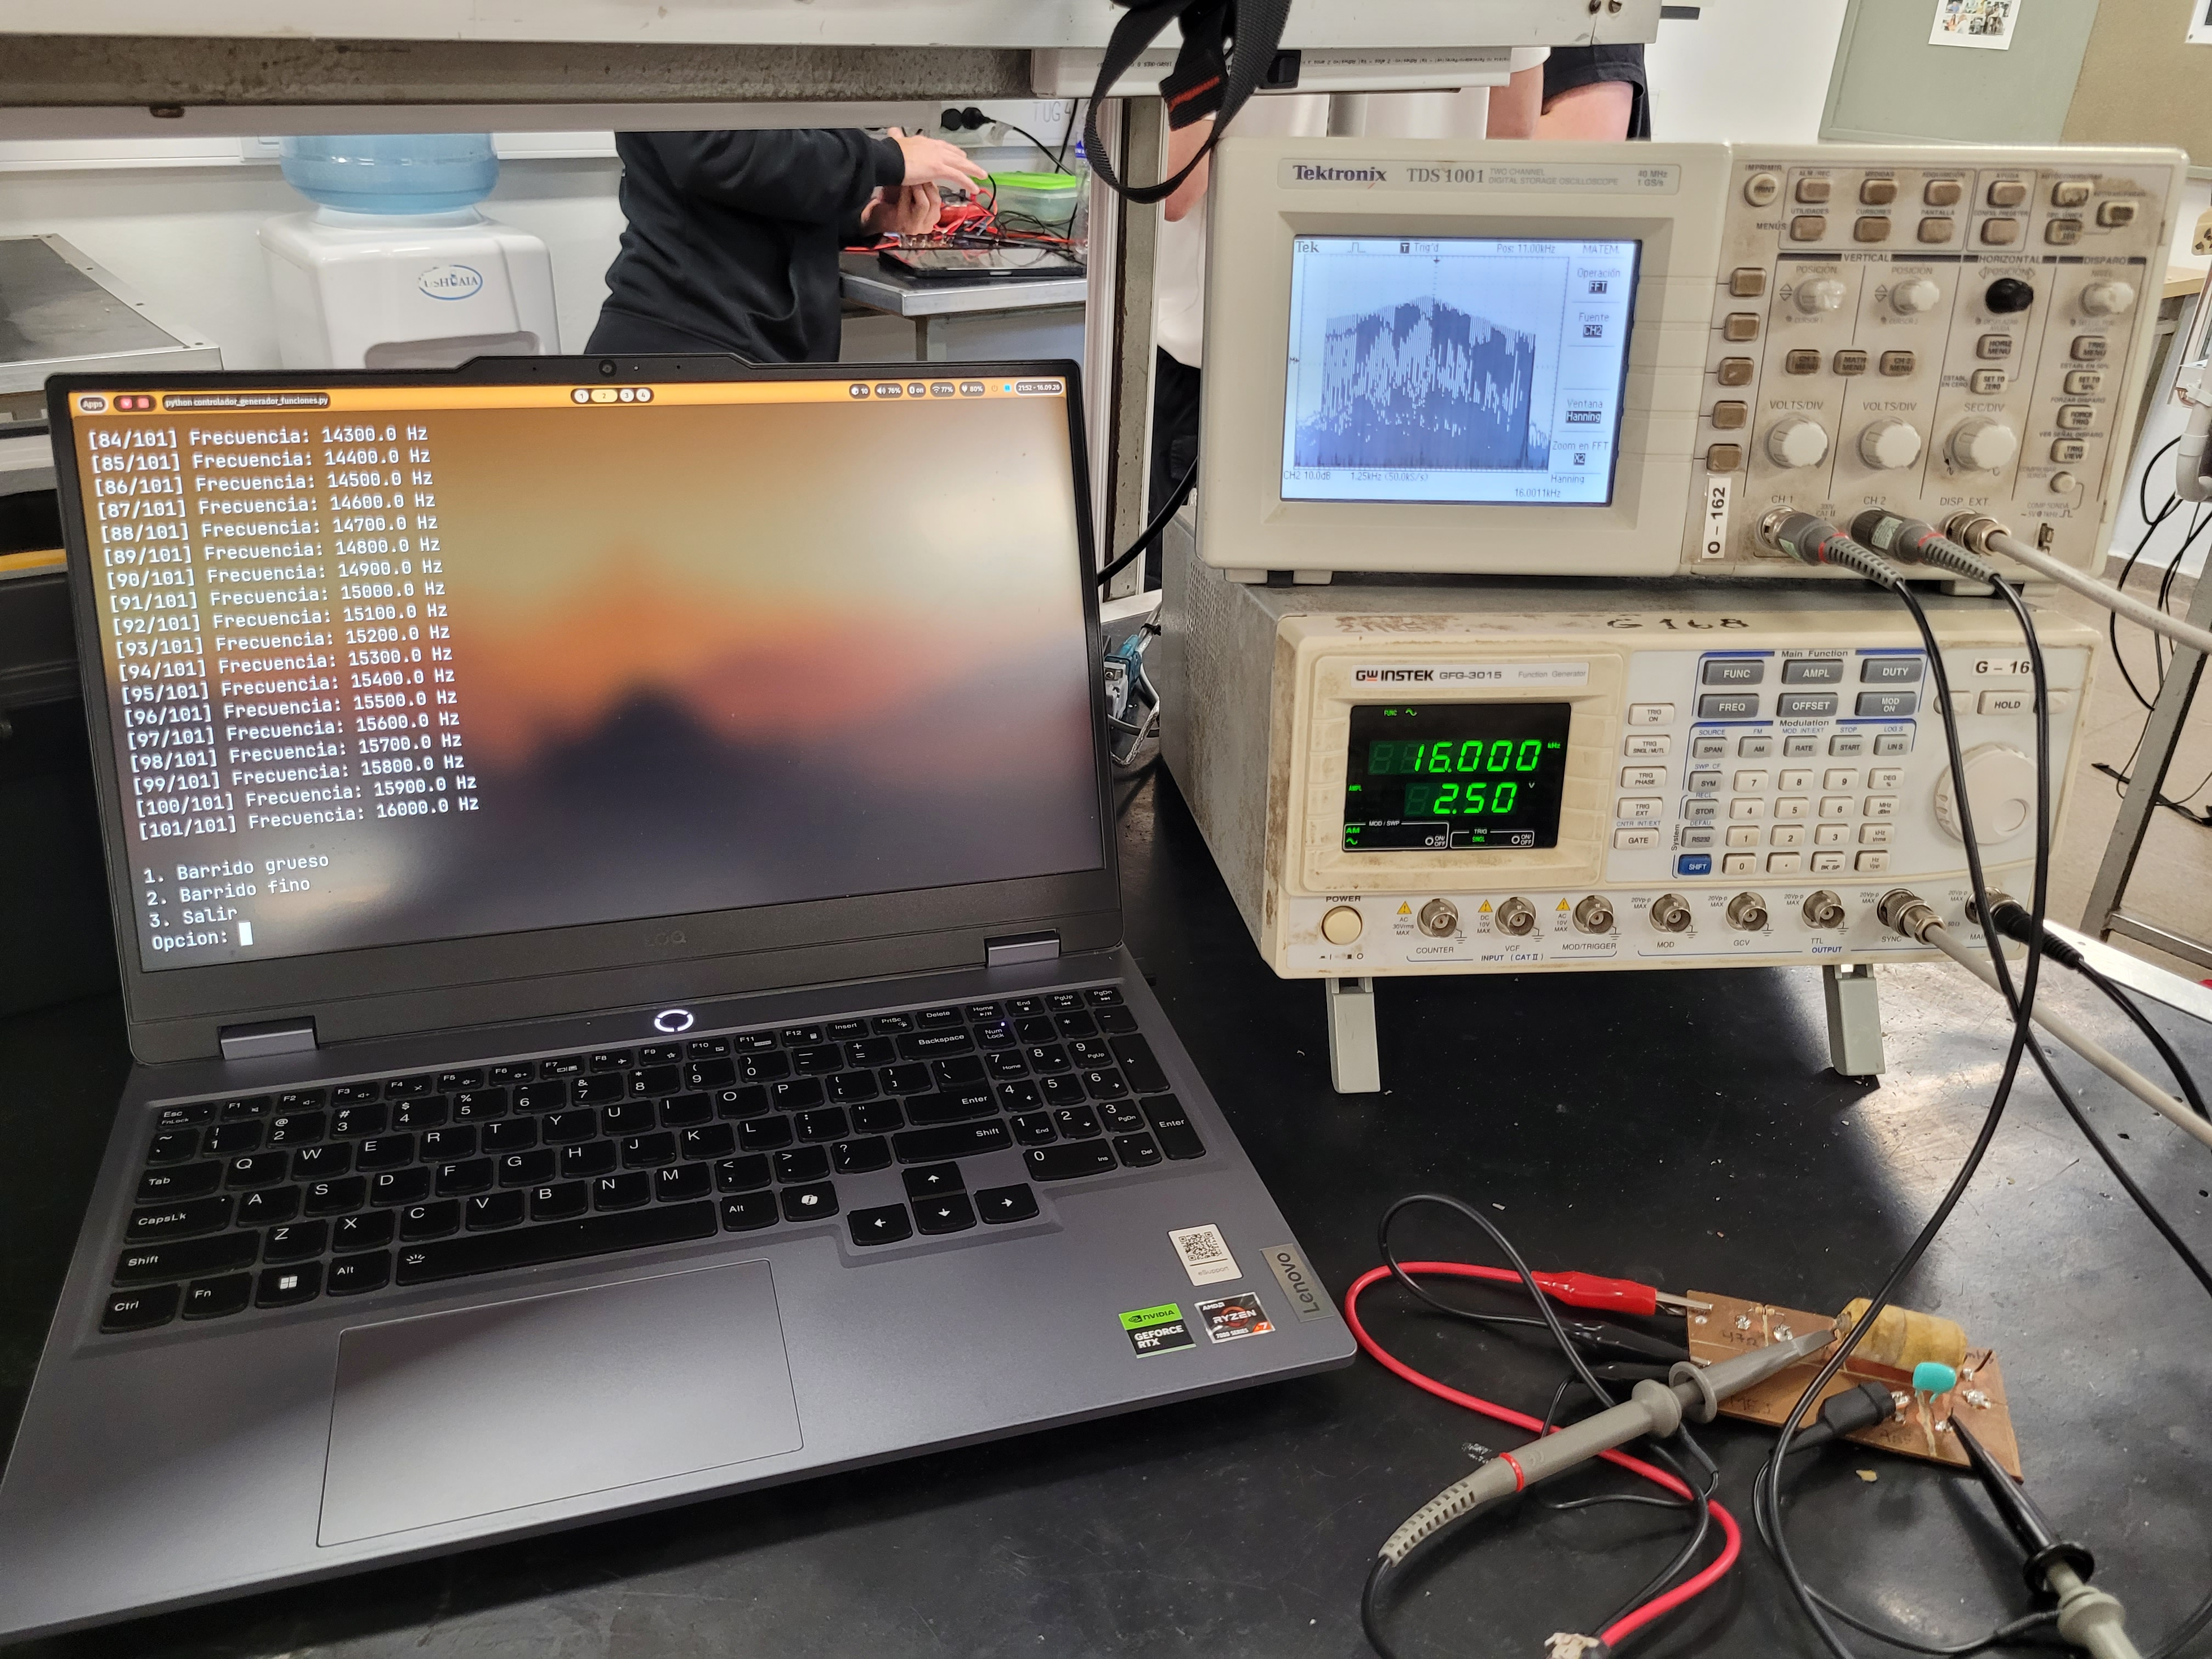
\includegraphics[width=\textwidth]{pictures/setup_fft_barrido_auto_corto.jpeg}
        \caption{Consola completando 101 pasos automáticos.}
        \label{fig.ej1:setup_fft_corto}
    \end{subfigure}
    \hfill
    \begin{subfigure}[t]{0.48\textwidth}
        \centering
        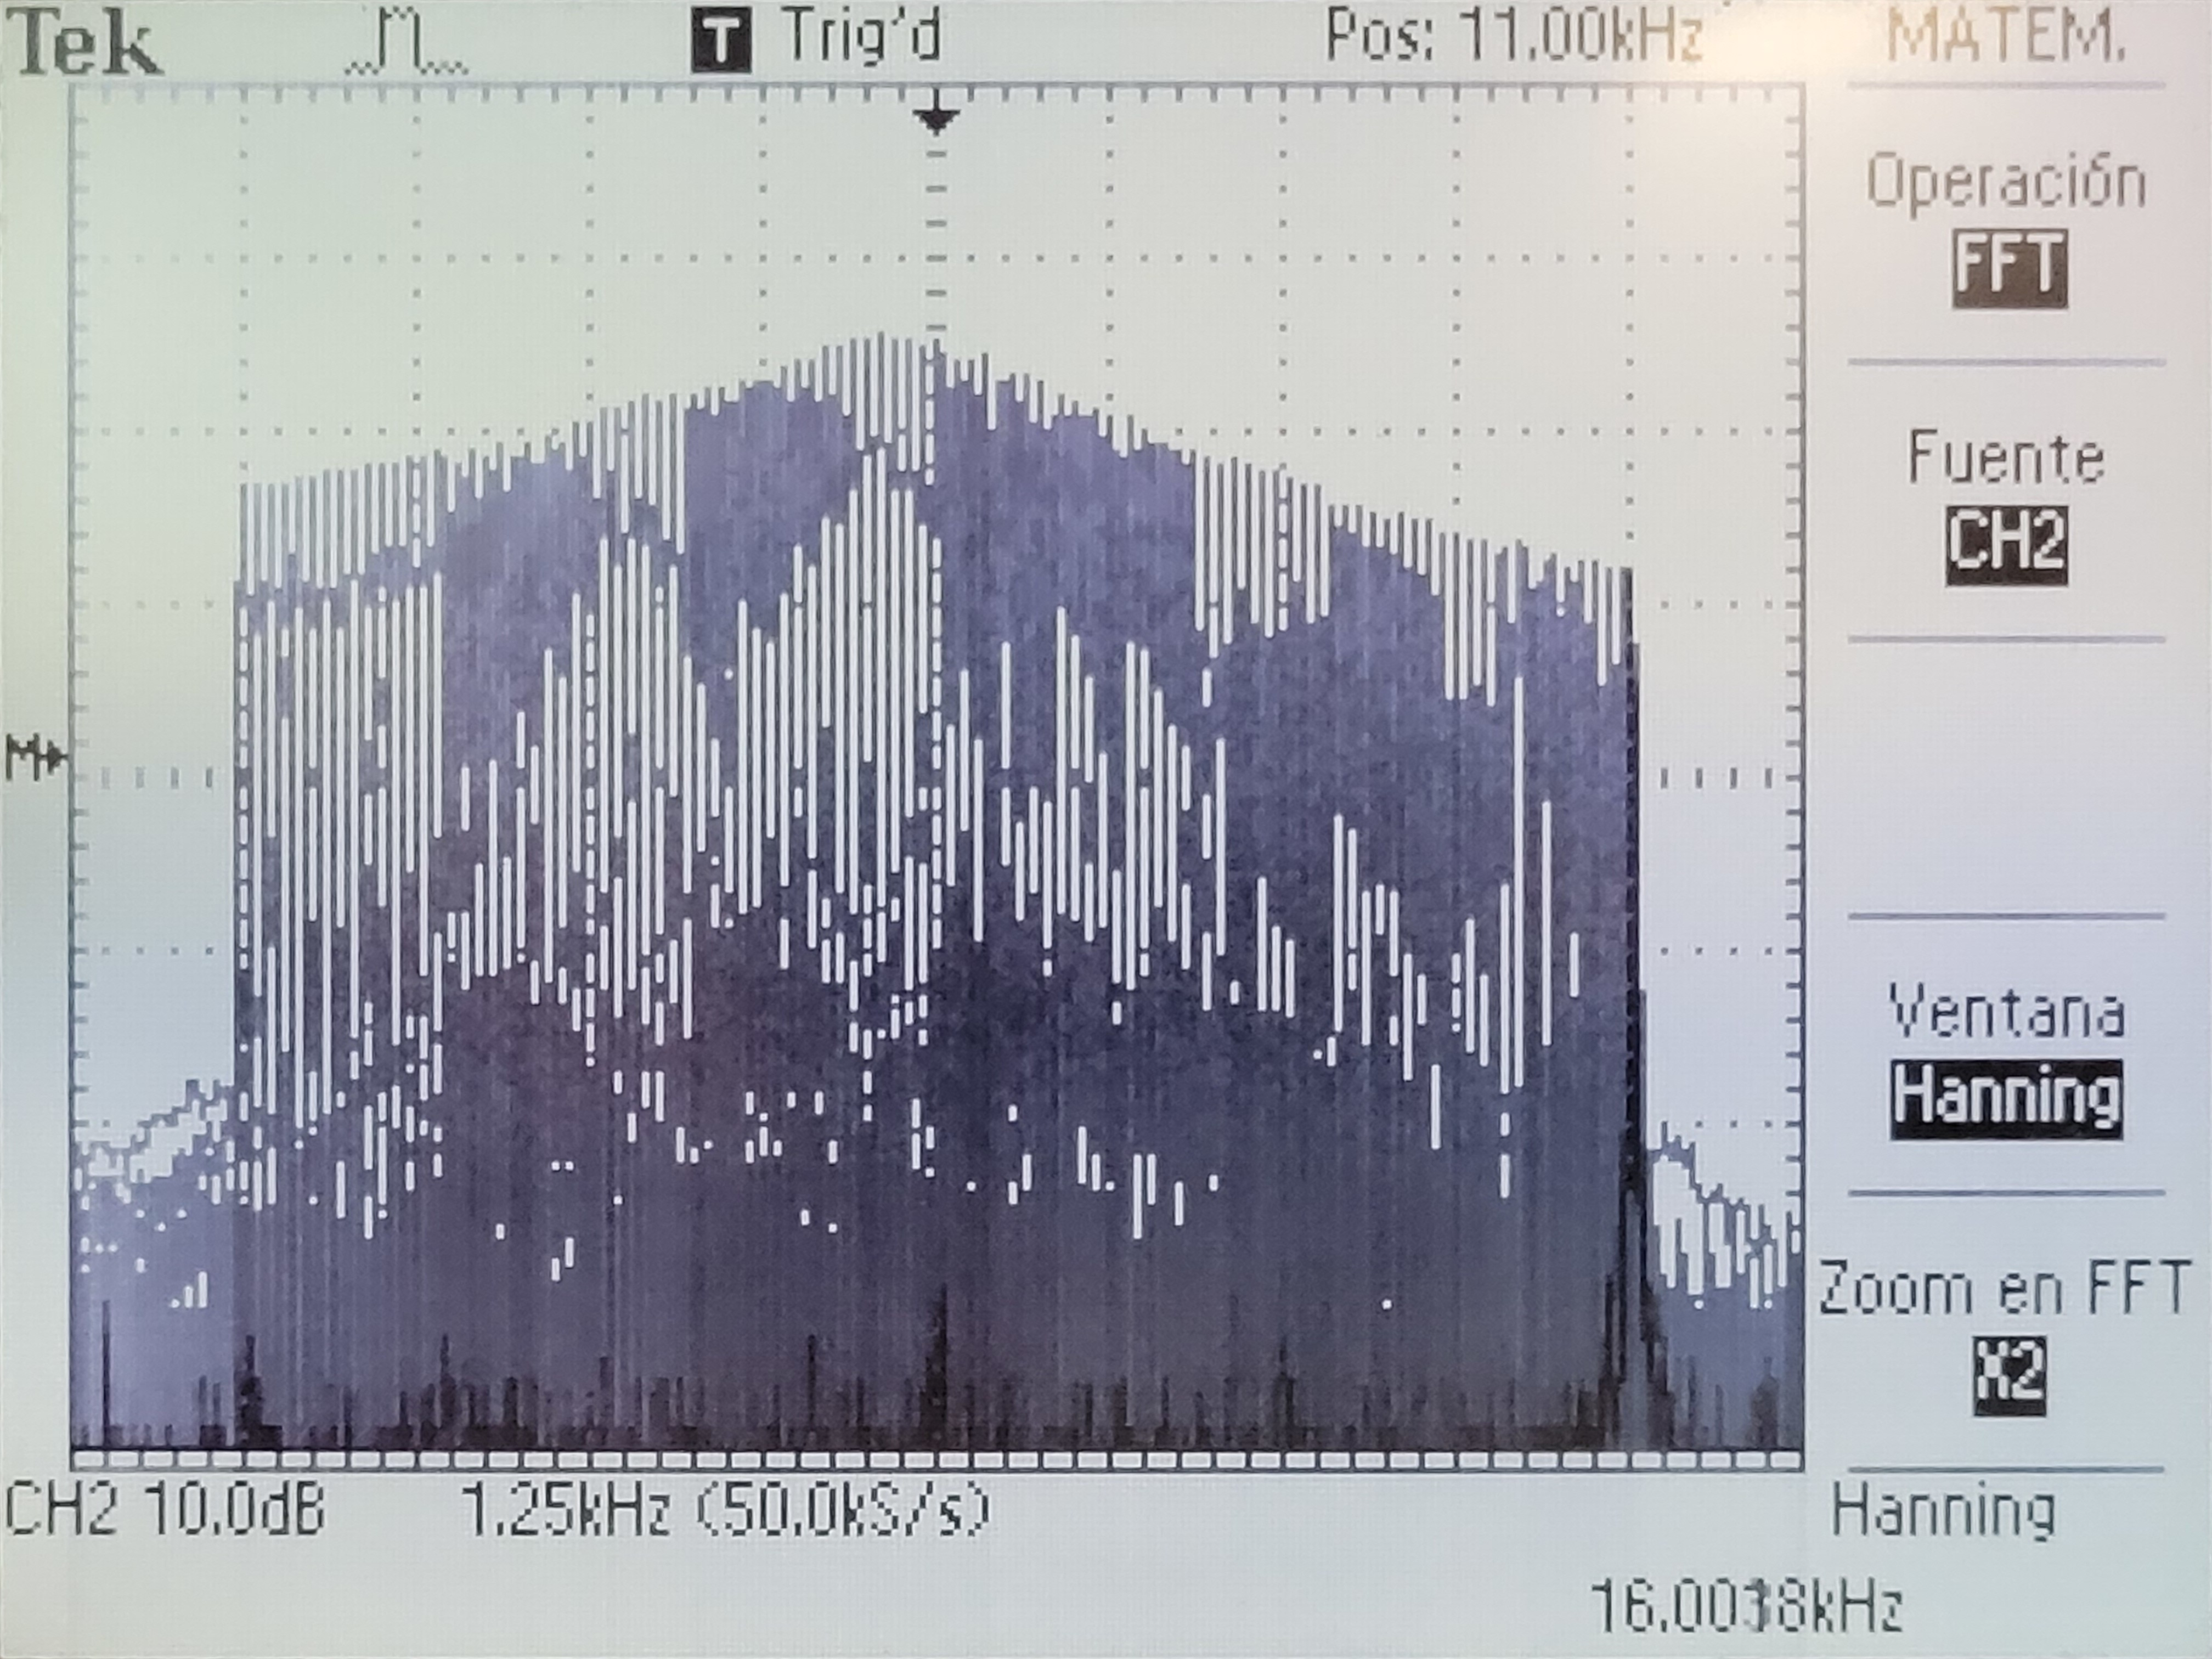
\includegraphics[width=\textwidth]{pictures/osc_fft_barrido_auto_corto.jpeg}
        \caption{Espectro FFT en CH2 centrado en $\qty{11.00}{\kilo\hertz}$.}
        \label{fig.ej1:osc_fft_corto}
    \end{subfigure}
    \caption{Validación espectral mediante barrido automático fino ($\qtyrange{6}{16}{\kilo\hertz}$, paso $\qty{100}{\hertz}$).}
    \label{fig.ej1:fft_corto}
\end{figure}

Se ejecutó tambien un barrido automático continuo de 101 pasos desde $\qty{6000}{\hertz}$ hasta $\qty{16000}{\hertz}$
con paso de $\qty{100}{\hertz}$ y un retardo de $\qty{1.0}{\second}$ por paso en la Figura~\ref{fig.ej1:fft_corto}. En
la pantalla del osciloscopio se aprecia con claridad la campana de resonancia del sistema, con el vértice de máxima
densidad espectral concentrado en torno a los $\qtyrange{10.7}{11.0}{\kilo\hertz}$ y un decrecimiento simétrico hacia
ambos extremos del intervalo.


  \chapter{Conclusiones}

Este trabajo práctico permitió implementar con éxito un sistema automatizado de medición y control
remoto de instrumental, integrando una computadora portátil, comunicación serie RS-232 y secuencias de
comandos SCPI para la caracterización completa de un circuito resonante serie RLC. A partir de los resultados obtenidos
y el análisis físico desarrollado, se extraen las siguientes conclusiones principales:

\begin{enumerate}
    \item \emph{Efectividad del control instrumental mediante SCPI y Python:} La arquitectura de software desarrollada
    en Python utilizando la biblioteca \texttt{pySerial} demostró robustez, estabilidad y flexibilidad operativa. La
    secuencia de inicialización estandarizada (\texttt{*IDN?}, \texttt{:FUNC:WAV}, \texttt{:AMPL:VOLT}, \texttt{:OFFSet})
    garantizó la repetibilidad de las condiciones iniciales del generador. La incorporación de modalidades de
    barrido automático y manual permitió tanto la exploración
    rápida de amplios rangos espectrales como la adquisición minuciosa y documentada de puntos singulares.
    \item \emph{Concordancia en la frecuencia de resonancia:} El valor experimental obtenido para la frecuencia de
    resonancia ($f_0 = \qty{10.70}{\kilo\hertz}$) presentó una concordancia notable con el valor teórico derivado de
    los parámetros nominales de la placa ($f_0^{\text{teo}} = \qty{10.98}{\kilo\hertz}$ para $L = \qty{30}{\milli\henry}$
    y $C = \qty{7}{\nano\farad}$), registrándose un error relativo de apenas $2.55\%$. Esta desviación reducida se
    encuentra completamente contenida dentro de las tolerancias constructivas habituales de componentes reactivos discretos.
    \item \emph{Validación espectral con FFT y persistencia infinita:} La utilización de la función matemática FFT con
    ventana Hanning acoplada a la persistencia infinita de pantalla permitió sintetizar la curva de transferencia
    global del filtro RLC entre $\qty{1}{\kilo\hertz}$ y $\qty{50}{\kilo\hertz}$. Cada pulso discreto inyectado por el
    barrido automático generó una línea espectral que, al acumularse en pantalla, delineó el perfil de ganancia
    pasa-banda y corroboró en el dominio frecuencial los parámetros temporales obtenidos.
\end{enumerate}



  \nocite{*}
  \printbibliography[heading=bibnumbered, title={Fuentes}]

  \chapter{Anexos Técnicos}

\section{Código Fuente del Software de Control en Python}
A continuación se transcribe el código fuente completo implementado en el script
\path{controlador_generador_funciones.py}, utilizado para la comunicación serie y la ejecución de los barridos de
frecuencia sobre el generador de funciones GW-Instek GFG-3015.

\lstinputlisting[
    style=python,
    language=Python,
    caption={Script de automatización y barrido en frecuencia mediante comandos SCPI.},
    label={list.ej1:codigo_control}
]{sources/controlador_generador_funciones.py}

\section{Comandos SCPI del Generador GW-Instek GFG-3015}
En la Tabla~\ref{tab.anexo:comandos_scpi} se resumen los principales comandos de la interfaz RS-232 implementados en
el generador GW-Instek GFG-3015 conforme al manual de usuario del fabricante~\cite{gwinstek_gfg3015}.

\begin{table}[!ht]
    \centering
    \small
    \begin{tabular}{|l|p{4.2cm}|l|p{4.5cm}|}
        \hline
        \textbf{Comando} & \textbf{Descripción} & \textbf{Parámetros} & \textbf{Función / Respuesta} \\ \hline
        \texttt{*IDN?} & Consulta de identificación & Ninguno & Devuelve fabricante, modelo y firmware. \\ \hline
        \texttt{*RST} & Reinicio del instrumento & Ninguno & Restablece parámetros de fábrica. \\ \hline
        \texttt{:FUNC:WAV} & Forma de onda & \texttt{1}, \texttt{2}, \texttt{3} & 1: Senoidal, 2: Triangular, 3: Cuadrada. \\ \hline
        \texttt{:AMPL:UNIT} & Unidad de amplitud & \texttt{1}, \texttt{2}, \texttt{3} & 1: $\mathrm{V_{pp}}$, 2: $\mathrm{V_{rms}}$, 3: $\mathrm{dBm}$. \\ \hline
        \texttt{:AMPL:VOLT} & Amplitud de salida & Numérico (NRf) & Ajusta la tensión sobre $\qty{50}{\ohm}$. \\ \hline
        \texttt{:OFFSet} & Offset continuo & Numérico (NRf) & Fija el nivel de continua en voltios. \\ \hline
        \texttt{:FREQ} & Frecuencia principal & Numérico (NRf) & Ajusta la frecuencia en Hertz. \\ \hline
        \texttt{:FREQ?} & Consulta de frecuencia & Ninguno & Devuelve el valor numérico en Hertz. \\ \hline
    \end{tabular}
    \caption{Conjunto principal de comandos SCPI para la interfaz serie del generador GFG-3015.}
    \label{tab.anexo:comandos_scpi}
\end{table}


\end{document}
